%
% A header that lets you compile a chapter by itself, or inside a larger document.
% Adapted from stackoverflow.com/questions/3655454/conditional-import-in-latex
%
%
%Use \inbpdocument and \outbpdocument in your individual files, in place of \begin{document} and \end{document}. In your main file, put in a \def \ismaindoc {} before including or importing anything.
%
% David Duvenaud
% June 2011
% 
% ======================================
%
%


\ifx\ismaindoc\undefined
	\newcommand{\inbpdocument}{
		\def \ismaindoc {}
		% Use this header if we are compiling by ourselves.
		\documentclass[a4paper,11pt,authoryear,index]{common/PhDThesisPSnPDF}
		
%\usepackage{draftwatermark}
%\SetWatermarkLightness{0.95}

% ******************************************************************************
% ****************************** Custom Margin *********************************

% Add `custommargin' in the document class options to use this section
% Set {innerside margin / outerside margin / topmargin / bottom margin}  and
% other page dimensions

\ifsetMargin
\else
    \RequirePackage[left=37mm,right=30mm,top=35mm,bottom=30mm]{geometry}
    \setFancyHdr % To apply fancy header after geometry package is loaded
\fi


%\chead{Unfinished draft}
%\cfoot{\texttt{Unfinished draft - compiled on \today{} at \currenttime}}

% *****************************************************************************
% ******************* Fonts (like different typewriter fonts etc.)*************

% Add `customfont' in the document class option to use this section

\ifsetFont
\else
    % Set your custom font here and use `customfont' in options. Leave empty to
    % load computer modern font (default LaTeX font).  

    \RequirePackage{libertine} 
\fi

% *****************************************************************************
% *************************** Bibliography  and References ********************

%\usepackage{cleveref} %Referencing without need to explicitly state fig /table

% Add `custombib' in the document class option to use this section
\ifsetBib % True, Bibliography option is chosen in class options
\else % If custom bibliography style chosen then load bibstyle here

   \RequirePackage[square, sort, numbers, authoryear]{natbib} % CustomBib

% If you would like to use biblatex for your reference management, as opposed to the default `natbibpackage` pass the option `custombib` in the document class. Comment out the previous line to make sure you don't load the natbib package. Uncomment the following lines and specify the location of references.bib file

% \RequirePackage[backend=biber, style=numeric-comp, citestyle=numeric, sorting=nty, natbib=true]{biblatex}
% \bibliography{References/references} %Location of references.bib only for biblatex

\fi


% changes the default name `Bibliography` -> `References'
\renewcommand{\bibname}{References}


% *****************************************************************************
% *************** Changing the Visual Style of Chapter Headings ***************
% Uncomment the section below. Requires titlesec package.

%\RequirePackage{titlesec}
%\newcommand{\PreContentTitleFormat}{\titleformat{\chapter}[display]{\scshape\Large}
%{\Large\filleft{\chaptertitlename} \Huge\thechapter}
%{1ex}{}
%[\vspace{1ex}\titlerule]}
%\newcommand{\ContentTitleFormat}{\titleformat{\chapter}[display]{\scshape\huge}
%{\Large\filleft{\chaptertitlename} \Huge\thechapter}{1ex}
%{\titlerule\vspace{1ex}\filright}
%[\vspace{1ex}\titlerule]}
%\newcommand{\PostContentTitleFormat}{\PreContentTitleFormat}
%\PreContentTitleFormat


% *****************************************************************************
% **************************** Custom Packages ********************************
% *****************************************************************************


% ************************* Algorithms and Pseudocode **************************

%\usepackage{algpseudocode} 


% ********************Captions and Hyperreferencing / URL **********************

% Captions: This makes captions of figures use a boldfaced small font. 
%\RequirePackage[small,bf]{caption}

\RequirePackage[labelsep=space,tableposition=top]{caption} 
%\renewcommand{\figurename}{Figure} %to support older versions of captions.sty
\captionsetup{labelsep = colon,belowskip=12pt,aboveskip=4pt}

% ************************ Formatting / Footnote *******************************

%\usepackage[perpage]{footmisc} %Range of footnote options 


% ****************************** Line Numbers **********************************

%\RequirePackage{lineno}
%\linenumbers

% ************************** Graphics and figures *****************************

%\usepackage{rotating}
%\usepackage{wrapfig}
%\usepackage{float}
\usepackage{subfig} %note: subfig must be included after the `caption` package. 


% ********************************* Table **************************************

%\usepackage{longtable}
%\usepackage{multicol}
%\usepackage{multirow}
%\usepackage{tabularx}


% ***************************** Math and SI Units ******************************

\usepackage{amsfonts}
\usepackage{amsmath}
\usepackage{amssymb}
%\usepackage{siunitx} % use this package module for SI units


% ******************************************************************************
% ************************* User Defined Commands ******************************
% ******************************************************************************

% *********** To change the name of Table of Contents / LOF and LOT ************

%\renewcommand{\contentsname}{My Table of Contents}
%\renewcommand{\listfigurename}{List of figures}
%\renewcommand{\listtablename}{List of tables}


% ********************** TOC depth and numbering depth *************************

\setcounter{secnumdepth}{2}
\setcounter{tocdepth}{2}

% ******************************* Nomenclature *********************************

% To change the name of the Nomenclature section, uncomment the following line

%\renewcommand{\nomname}{Symbols}


% ********************************* Appendix ***********************************

% The default value of both \appendixtocname and \appendixpagename is `Appendices'. These names can all be changed via: 

%\renewcommand{\appendixtocname}{List of appendices}
%\renewcommand{\appendixname}{Appndx}

		% All my custom preamble stuff.  Shouldn't overlap with anything in official-preamble




% Paths to figure and table directories.
\newcommand{\symmetryfigsdir}{figures/symmetries}
\newcommand{\topologyfiguresdir}{figures/topology}
\newcommand{\infinitefiguresdir}{figures/infinite}
\newcommand{\grammarfiguresdir}{figures/grammar}
\newcommand{\introfigsdir}{figures/intro}
\newcommand{\gplvmfiguresdir}{figures/gplvm}
\newcommand{\warpedfiguresdir}{figures/warped-mixtures}
\newcommand{\deeplimitsfiguresdir}{figures/deep-limits}
\newcommand{\quadraturefigsdir}{figures/quadrature}
\newcommand{\additivefigsdir}{figures/additive}
\newcommand{\decompfigsdir}{figures/decomp}
\newcommand{\examplefigsdir}{figures/worked-example}

\usepackage{bm}  % for warped mixtures - is this necessary?
\usepackage{booktabs}
\usepackage{tabularx}
\usepackage{multirow}
\usepackage{datetime}
\renewcommand{\tabularxcolumn}[1]{>{\arraybackslash}m{#1}}
\usepackage{relsize}
\usepackage{graphicx}
\usepackage{amsmath,amssymb,textcomp}
\usepackage{nicefrac}
\usepackage{amsthm}
\usepackage{tikz}
\usetikzlibrary{arrows}
\usetikzlibrary{calc}
\usepackage{nth}
\usepackage{rotating}
\usepackage{array}
\usepackage{fp}
\usepackage{cleveref}   % Note: this package sometimes causes the page counter to reset.
\crefname{equation}{equation}{equations}
\crefname{figure}{figure}{figures}
%\usepackage{common/sectsty}

% Controls capitalization of all headers
%\usepackage{stringstrings}
%\usepackage[explicit]{titlesec}
%\newcommand\SentenceCase[1]{%
%  \caselower[e]{#1}%
%  \capitalize[q]{\thestring}%
%}
%\titleformat{\section}
%  {\normalfont\Large\bfseries}{\thesection}{1em}{\SentenceCase{#1}\thestring}


%\titleformat{\section} % The normal, unstarred version
%    {\Large\bfseries}{}{2ex}
%    {\thesection. \MakeSentenceCase{#1}}

%\titleformat{name=\section,numberless} % The starred version; note the `numberless` key
%    {\Large\bfseries}{}{2ex}
%    {\MakeSentenceCase{#1}}

\usepackage[hyperpageref]{backref}
% Setup to show (pages 4 and 9) sort of thing in the bibliography - DD
%\def\foo{\hspace{\fill}\mbox{}\linebreak[0]\hspace*{\fill}}
%\def\foo{\parbox{3cm}{\hfill}
%\def\foo{\parbox{3cm}{\hfill}
%\newcommand\foo[1]{{\raggedleft{\hfill{\mbox{\hfill{#1}}}}}}
\newcommand{\comfyfill}[1]{% = Thorsten Donig's \signed
  \unskip\hspace*{0.1em plus 1fill}
  \nolinebreak[3]%
  \hspace*{\fill}\mbox{#1}
  \parfillskip0pt\par
}
\newcommand\foo[1]{{\comfyfill{\mbox{#1}}}}
%\newcommand\foo[1]{{\mbox{#1}}}
\renewcommand*{\backref}[1]{}
\renewcommand*{\backrefalt}[4]{%
\ifcase #1 %
%
\or
\foo{(page #2)}%
\else
\foo{(pages #2)}%
\fi
}

\usepackage{stringstrings}

%\newcommand{\headercase}{\
%\DeclareFieldFormat{titlecase}{\MakeSentenceCase{#1}}


%% For submission, make all render blank.
%%%%%%%%%%%%%%%%%%%%%%%%%%%%%%%%%%%%%%%%%%%%%%%%%%%%%%%%%%
%%%% EDITING HELPER FUNCTIONS  %%%%%%%%%%%%%%%%%%%%%%%%%%%
%%%%%%%%%%%%%%%%%%%%%%%%%%%%%%%%%%%%%%%%%%%%%%%%%%%%%%%%%%

%% NA: needs attention (rough writing whose correctness needs to be verified)
%% TBD: instructions for how to fix a gap ("Describe the propagation by ...")
%% PROBLEM: bug or missing crucial bit 

%% use \fXXX versions of these macros to put additional explanation into a footnote.  
%% The idea is that we don't want to interrupt the flow of the paper or make it 
%% impossible to read because there are a bunch of comments.

%% NA's (and TBDs, those less crucially) should be written so 
%% that they flow with the text.

\definecolor{WowColor}{rgb}{.75,0,.75}
\definecolor{SubtleColor}{rgb}{0,0,.50}

% inline
\newcommand{\NA}[1]{\textcolor{SubtleColor}{ {\tiny \bf ($\star$)} #1}}
\newcommand{\LATER}[1]{\textcolor{SubtleColor}{ {\tiny \bf ($\dagger$)} #1}}
\newcommand{\TBD}[1]{\textcolor{SubtleColor}{ {\tiny \bf (!)} #1}}
\newcommand{\PROBLEM}[1]{\textcolor{WowColor}{ {\bf (!!)} {\bf #1}}}

% as margin notes

\newcounter{margincounter}
\newcommand{\displaycounter}{{\arabic{margincounter}}}
\newcommand{\incdisplaycounter}{{\stepcounter{margincounter}\arabic{margincounter}}}

\newcommand{\fTBD}[1]{\textcolor{SubtleColor}{$\,^{(\incdisplaycounter)}$}\marginpar{\tiny\textcolor{SubtleColor}{ {\tiny $(\displaycounter)$} #1}}}

\newcommand{\fPROBLEM}[1]{\textcolor{WowColor}{$\,^{((\incdisplaycounter))}$}\marginpar{\tiny\textcolor{WowColor}{ {\bf $\mathbf{((\displaycounter))}$} {\bf #1}}}}

\newcommand{\fLATER}[1]{\textcolor{SubtleColor}{$\,^{(\incdisplaycounter\dagger)}$}\marginpar{\tiny\textcolor{SubtleColor}{ {\tiny $(\displaycounter\dagger)$} #1}}}

%\renewcommand{\LATER}[1]{}
%\renewcommand{\fLATER}[1]{}
%\renewcommand{\TBD}[1]{}
%\renewcommand{\fTBD}[1]{}
%\renewcommand{\PROBLEM}[1]{}
%\renewcommand{\fPROBLEM}[1]{}
%\renewcommand{\NA}[1]{}


% HUMBLE WORDS: shown slightly smaller when in normal text
% Thanks to Christian Steinruecken!

% HUMBLE WORDS: shown slightly smaller when in normal text
% Christian Steinruecken
%
\makeatletter%
%\def\@humbleformat#1{{\fontsize{}{1em}\selectfont #1}}
%\def\@humbleformat#1{\textsmaller{#1}}%
\newlength{\nonHumbleHeight}
\def\@humbleformat#1{{\settoheight{\nonHumbleHeight}{#1}\resizebox{!}{0.94\nonHumbleHeight}{#1}}}%
\def\@idxhumbleformat#1{{\relscale{0.95}{#1}}}%
%\def\@humbleformat#1{{#1}}%
\def\declareHumble#1#2{%
  \expandafter\def\csname #1\endcsname{\@humbleformat{#2}}%
  \expandafter\def\csname s#1\endcsname{{#2}}%
  \expandafter\def\csname idx#1\endcsname{{\@idxhumbleformat{#2}}}%
}%
\def\humble#1{\@humbleformat{#1}}%
\def\idxhumble#1{\@idxhumbleformat{#1}}%
\makeatother%

% Convenient indexing for humble abbreviations
\def\humbleindex#1#2{\index{#1@\idxhumble{#1}}}



% TODO: Clean up duplicates
\declareHumble{ANOVA}{ANOVA}
\declareHumble{ARD}{ARD}
\declareHumble{BIC}{BIC}
\declareHumble{BMC}{BMC}
\declareHumble{bq}{BQ}
\declareHumble{CRP}{CRP}
\declareHumble{dirpro}{DP}
\declareHumble{HDMR}{HDMR}
\declareHumble{GAM}{GAM}
\declareHumble{GEM}{GEM}
\declareHumble{GMM}{GMM}
\declareHumble{gplvm}{GP-LVM}
\declareHumble{gpml}{GPML}
\declareHumble{GPML}{GPML}
\declareHumble{gprn}{GPRN}
\declareHumble{gpt}{GP}
\declareHumble{gp}{GP}
\declareHumble{HKL}{HKL}
\declareHumble{HMC}{HMC}
\declareHumble{ibp}{IBP}
\declareHumble{iGMM}{iGMM}
\declareHumble{iwmm}{iWMM}
\declareHumble{kCP}{CP}
\declareHumble{kCW}{CW}
\declareHumble{kC}{C}
\declareHumble{KDE}{KDE}
\declareHumble{kLin}{Lin}
\declareHumble{KPCA}{KPCA}
\declareHumble{kPer}{Per}
\declareHumble{kPerGen}{ZMPer}
\declareHumble{kRQ}{RQ}
\declareHumble{kSE}{SE}
\declareHumble{kWN}{WN}
\declareHumble{Lin}{Lin}
\declareHumble{LBFGS}{L-BFGS}
\declareHumble{LIBSVM}{LIBSVM}
\declareHumble{MAP}{MAP}
\declareHumble{mcmc}{MCMC}
\declareHumble{MKL}{MKL}
\declareHumble{MLP}{MLP}
\declareHumble{MNIST}{MNIST}
\declareHumble{MSE}{MSE}
\declareHumble{OU}{OU}
\declareHumble{Per}{Per}
\declareHumble{RBF}{RBF}
\declareHumble{RMSE}{RMSE}
\declareHumble{RQ}{RQ}
\declareHumble{SBQ}{SBQ}
\declareHumble{seard}{SE-ARD}
\declareHumble{sefull}{SE-\textnormal{full}}
\declareHumble{SEGP}{SE-GP}
\declareHumble{SE}{SE}
\declareHumble{SNR}{SNR}
\declareHumble{SSANOVA}{SS-ANOVA}
\declareHumble{SVM}{SVM}
\declareHumble{UCI}{UCI}
\declareHumble{UMIST}{UMIST}
\declareHumble{vbgplvm}{VB GP-LVM}

\newcommand{\kSig}{\boldsymbol\sigma}

\def\subexpr{{\cal S}}
\def\baseker{{\cal B}}
\def\numWinners{k}

\def\ie{i.e.\ }
\def\eg{e.g.\ }
\def\etc{etc.\ }
\let\oldemptyset\emptyset
%\let\emptyset 0




% Unify notation between neural-net land and GP-land.
\newcommand{\hphi}{h}
\newcommand{\hPhi}{\vh}
\newcommand{\walpha}{w}
\newcommand{\wboldalpha}{\bw}
\newcommand{\wcapalpha}{\vW}
\newcommand{\lengthscale}{w}

\newcommand{\layerindex}{\ell}



\newcommand{\gpdrawbox}[1]{
\setlength\fboxsep{0pt}
\hspace{-0.15in} 
\fbox{
\includegraphics[width=0.464\columnwidth]{\deeplimitsfiguresdir/deep_draws/deep_gp_sample_layer_#1}
}}



\newcommand{\procedurename}{ABCD}
\newcommand{\genText}[1]{{\sf #1}}



\newcommand{\asdf}{$^{\textnormal{th}}$}

\newcommand{\binarysum}{\sum_{\bf{x} \in \{0,1\}^D}}
\newcommand{\expect}{\mathbb{E}}
\newcommand{\expectargs}[2]{\mathbb{E}_{#1} \left[ {#2} \right]}
\newcommand{\var}{\mathbb{V}}
\newcommand{\varianceargs}[2]{\mathbb{V}_{#1} \left[ {#2} \right]}
\newcommand{\cov}{\operatorname{cov}}
\newcommand{\Cov}{\operatorname{Cov}}
\newcommand{\covargs}[2]{\Cov \left[ {#1}, {#2} \right]}
\newcommand{\variance}{\mathbb{V}}
\newcommand{\vecop}[1]{\operatorname{vec} \left( {#1} \right)}

\newcommand{\covarianceargs}[2]{\Cov_{#1} \left[ {#2} \right]}
\newcommand{\colvec}[2]{\left[ \begin{array}{c} {#1} \\ {#2} \end{array} \right]}
\newcommand{\tbtmat}[4]{\left[ \begin{array}{cc} {#1} & {#2} \\ {#3} & {#4} \end{array} \right]}

\newcommand{\acro}[1]{{\humble{#1}}}
%\newcommand{\vect}[1]{\boldsymbol{#1}}
\newcommand{\vect}[1]{{\bf{#1}}}
\newcommand{\mat}[1]{\mathbf{#1}}
\newcommand{\pderiv}[2]{\frac{\partial #1}{\partial #2}}
\newcommand{\npderiv}[2]{\nicefrac{\partial #1}{\partial #2}}

\newcommand{\pha}{^{\phantom{:}}}

\newcommand{\argmin}{\operatornamewithlimits{argmin}}
\newcommand{\argmax}{\operatornamewithlimits{argmax}}

% The following designed for probabilities with long arguments

\newcommand{\Prob}[2]{P\!\left(\,#1\;\middle\vert\;#2\,\right)}
\newcommand{\ProbF}[3]{P\!\left(\,#1\!=\!#2\;\middle\vert\;#3\,\right)}
\newcommand{\p}[2]{p\!\left(#1\middle\vert#2\right)}
\newcommand{\po}[1]{p\!\left(#1\right)}
\newcommand{\pF}[3]{p\!\left(\,#1\!=\!#2\;\middle\vert\;#3\,\right)} 
\newcommand{\mean}[2]{{m}\!\left(#1\middle\vert#2\right)}



\newcommand{\valpha}{\boldsymbol{\alpha}}
\newcommand{\va}{\vect{a}}
\newcommand{\vA}{\vect{A}}
\newcommand{\vB}{\mat{B}}
\newcommand{\vb}{\vect{b}}
\newcommand{\vC}{\mat{C}}
\newcommand{\vc}{\vect{c}}
\newcommand{\vecf}{\boldsymbol{f}}
\newcommand{\vell}{\vect{\ell}}
\newcommand{\vepsilon}{\boldsymbol{\epsilon}}
\newcommand{\veps}{\boldsymbol{\epsilon}}
\newcommand{\ve}{\boldsymbol{\epsilon}}
\newcommand{\vf}{\vecf}
\newcommand{\vg}{\vect{g}}
\newcommand{\vh}{\vect{h}}
\newcommand{\vI}{\mat{I}}
\newcommand{\vK}{\mat{K}}
\newcommand{\vk}{\vect{k}}
\newcommand{\vL}{\mat{L}}
\newcommand{\vl}{\vect{l}}
\newcommand{\vmu}{{\boldsymbol{\mu}}}
\newcommand{\vone}{\vect{1}}
\newcommand{\vphi}{{\boldsymbol{\phi}}}
\newcommand{\vpi}{{\boldsymbol{\pi}}}
\newcommand{\vq}{\vect{q}}
\newcommand{\vR}{\mat{R}}
\newcommand{\vr}{\vect{r}}
\newcommand{\vsigma}{{\boldsymbol{\sigma}}}
\newcommand{\vSigma}{\mat{\Sigma}}
\newcommand{\vS}{\mat{S}}
\newcommand{\vs}{\vect{s}}
\newcommand{\vtheta}{{\boldsymbol{\theta}}}
\newcommand{\vu}{\vect{u}}
\newcommand{\vV}{\mat{V}}
\newcommand{\vW}{\mat{W}}
\newcommand{\vw}{\vect{w}}
\newcommand{\vX}{\mat{X}}
\newcommand{\vx}{\vect{x}}
\newcommand{\vY}{\mat{Y}}
\newcommand{\vy}{\vect{y}}
\newcommand{\vzero}{\vect{0}}
\newcommand{\vZ}{\mat{Z}}
\newcommand{\vz}{\vect{z}}


% deep gp notation
\newcommand{\netweights}{w}
\newcommand{\vnetweights}{\vw}
\newcommand{\mnetweights}{\vW}
\newcommand{\outweights}{\v}
\newcommand{\voutweights}{\vv}
\newcommand{\moutweights}{\vV}

\newcommand{\unitparams}{\v}
\newcommand{\vunitparams}{\vv}
\newcommand{\munitparams}{\vV}


\newcommand{\He}{\mathcal{H}}
\newcommand{\normx}[2]{\left\|#1\right\|_{#2}}
\newcommand{\Hnorm}[1]{\normx{#1}{\He}}
\newcommand{\mmd}{{\rm MMD}}


\newcommand{\mf}{\bar{\vf}}

%\newcommand{\mf}{\mu} %{\bar{\ell}}
\newcommand{\lf}{f} % Likelihood function
\newcommand{\st}{_\star}

% from simpler log-bq writeup
\newcommand{\lftwo}{{\log \ell}}
\newcommand{\mftwo}{{\bar \ell}}
\newcommand{\loggp}{{\log\acro{GP}}}%| \bX, \vy )}}
\newcommand{\loggpdist}{{\acro{GP}(\lftwo)}}%| \vX, \vy )}}


\newcommand{\inv}{^{{\mathsmaller{-1}}}}
\newcommand{\tohalf}{^{{\mathsmaller{\nicefrac{1}{2}}}}}

\newcommand{\Normal}{\mathcal{N}}
\newcommand{\N}[3]{\mathcal{N}\!\left(#1 \middle| #2,#3\right)}
\newcommand{\Nt}[2]{\mathcal{N}\!\left(#1,#2\right)}
\newcommand{\NT}[2]{\mathcal{N}\!\left(#1,#2\right)}
\newcommand{\GPdist}[3]{\mathcal{GP}\!\left(#1 \, \middle| \, #2, #3 \right)}
\newcommand{\GPdisttwo}[2]{\mathcal{GP}\!\left(\, #1, #2 \right)}
\newcommand{\bN}[3]{\mathcal{N}\big(#1 \middle| #2,#3\big)}
\newcommand{\boldN}[3]{\text{\textbf{\mathcal{N}}}\big(#1;#2,#3\big)}
\newcommand{\ones}[1]{\mat{1}_{#1}}
\newcommand{\eye}[1]{\mat{E}_{#1}}
\newcommand{\tra}{^{\mathsf{T}}}
%\newcommand{\tra}{^{\top}}
%\mathsf{T}
\newcommand{\trace}{\operatorname{tr}}
\newcommand{\shift}{\operatorname{shift}}
\renewcommand{\mod}{\operatorname{mod}}
\newcommand{\deq}{:=}
\newcommand{\oneofk}{\operatorname{one-of-k}}
%\newcommand{\degree}{^\circ}

\newcommand{\GPt}[2]{\mathcal{GP}\!\left(#1,#2\right)}
%\newcommand{\GPt}[2]{\gp\!\left(#1,#2\right)}

\DeclareMathOperator{\tr}{tr}
\DeclareMathOperator{\chol}{chol}
\DeclareMathOperator{\diag}{diag}

\newenvironment{narrow}[2]{%
  \begin{list}{}{%
  \setlength{\topsep}{0pt}%
  \setlength{\leftmargin}{#1}%
  \setlength{\rightmargin}{#2}%
  \setlength{\listparindent}{\parindent}%
  \setlength{\itemindent}{\parindent}%
  \setlength{\parsep}{\parskip}}%
\item[]}{\end{list}}



\newcommand{\dist}{\ \sim\ }
\def\given{\,|\,}

% Table stuff
\newcolumntype{C}[1]{>{\centering\let\newline\\\arraybackslash\hspace{0pt}}m{#1}}
\newcolumntype{L}[1]{>{\raggedright\let\newline\\\arraybackslash\hspace{0pt}}m{#1}}
\newcolumntype{R}[1]{>{\raggedleft\let\newline\\\arraybackslash\hspace{0pt}}m{#1}}

\newcommand{\defeq}{\mathrel{:\mkern-0.25mu=}}

\def\ie{i.e.\ }
\def\eg{e.g.\ }
\def\iid{i.i.d.\ }
%\def\simiid{\sim_{\mbox{\tiny iid}}}
\def\simiid{\overset{\mbox{\tiny iid}}{\sim}}
\def\simind{\overset{\mbox{\tiny \textnormal{ind}}}{\sim}}
\def\eqdist{\stackrel{\mbox{\tiny d}}{=}}
%\newcommand{\distas}[1]{\mathbin{\overset{#1}{\kern \z@ \sim}}}
%TODO: fix this - it worked outside the thesis!
\newcommand{\distas}[1]{\mathbin{\overset{#1}{\sim}}}

\def\Reals{\mathbb{R}}

\def\Uniform{\mbox{\rm Uniform}}
\def\Bernoulli{\mbox{\rm Bernoulli}}
\def\GP{\mathcal{GP}}
\def\GPLVM{\mathcal{GP-LVM}}




% Kernel stuff

\def\iva{\vect{\inputVar}}
\def\ivaone{\inputVar}
\def\inputVar{x}
\def\InputVar{X}
\def\InputSpace{\mathcal{X}}
\def\outputVar{y}
\def\OutputSpace{\mathcal{Y}}
\def\function{f}
\def\kernel{k}
\def\KernelMatrix{K}
\def\SumKernel{\sum}
\def\ProductKernel{\prod}
\def\expression{e}
\def\feat{\vh}

\newcommand{\kerntimes}{ \! \times \!}
\newcommand{\kernplus}{ \, + \,}


% Proof stuff
\theoremstyle{plain}
\newtheorem{theorem}{Theorem}[section]
\newtheorem{lemma}[theorem]{Lemma}
\newtheorem{prop}[theorem]{Proposition}
\newtheorem{proposition}{Proposition}
\newtheorem*{cor}{Corollary}

% For infinite bq
\newcommand{\iv}{\theta}
\newcommand{\viv}{\vtheta}

% For intro chapter
\newcommand{\funcval}{\vf(\vX)}
\newcommand{\testpoint}{{\vx^\star}}

\newcommand{\underwrite}[2]{{\underbrace{#1}_{\textnormal{#2}}}}



% For kernel figures
\newcommand{\fhbig}{2cm}%
\newcommand{\fwbig}{3cm}%
\newcommand{\kernpic}[1]{\includegraphics[height=\fhbig,width=\fwbig]{\grammarfiguresdir/structure_examples/#1}}%
\newcommand{\kernpicr}[1]{\rotatebox{90}{\includegraphics[height=\fwbig,width=\fhbig]{\grammarfiguresdir/structure_examples/#1}}}%
\newcommand{\addkernpic}[1]{{\includegraphics[height=\fhbig,width=\fwbig]{\grammarfiguresdir/additive_multi_d/#1}}}%
\newcommand{\largeplus}{\tabbox{{\Large+}}}%
\newcommand{\largeeq}{\tabbox{{\Large=}}}%
\newcommand{\largetimes}{\tabbox{{\Large$\times$}}}%
\newcommand{\fixedx}{$x$ (with $x' = 1$)}%

% for warped mixtures
\newcommand{\CLAS}{\vz}  %cluster assignments
\newcommand{\CLASi}{z} % individual cluster assignments


		% ************************ Thesis Information & Meta-data **********************

%% The title of the thesis
\title{Automating statistical modelling}

%\texorpdfstring is used for PDF metadata. Usage:
%\texorpdfstring{LaTeX_Version}{PDF Version (non-latex)} eg.,
%\texorpdfstring{$sigma$}{sigma}

%% The full name of the author
\author{James Robert Lloyd}

%% Department (eg. Department of Engineering, Maths, Physics)
%\dept{Department of Engineering}

%% University and Crest
\university{University of Cambridge}
\crest{
\includegraphics[width=0.25\textwidth]{misc/University_Crest}}

%% You can redefine the submission text:
% Default as per the University guidelines: This dissertation is submitted for
% the degree of Doctor of Philosophy
%\renewcommand{\submissiontext}{change the default text here if needed}

%% Full title of the Degree 
\degree{Doctor of Philosophy}
 
%% College affiliation (optional)
\college{Trinity College}

%% Submission date
\degreedate{December 2014} 

%% Meta information
\subject{Machine Learning}
\keywords{{LaTeX} {PhD Thesis} {Engineering} {University of Cambridge} {Machine Learning} {Gaussian processes} {Time Series} {Model checking} {Model criticism} {Aldous--Hoover} {Networks}}



		\begin{document}
	}	
	\newcommand{\outbpdocument}[1]{
		% Fake chapters so references aren't broken
		\label{ch:intro}                
		\label{ch:dummy}
		\label{ch:discussion}
		%\bibliographystyle{common/CUEDthesis}
		\bibliographystyle{plainnat}
		\bibliography{references.bib}
		\end{document}
	}	
\else
	%If we're inside another document, no need to re-start the document.
	\ifx\inbpdocument\undefined
		\newcommand{\inbpdocument}{}
		\newcommand{\outbpdocument}[1]{}
	\fi
\fi

\inbpdocument

\chapter{Statistical models for networks}
\label{ch:networks}

In much of the machine learning literature to date, data can naturally be viewed as a sequence or a list.
Of course, there are many other types and structures of data, such as those which are most naturally represented as a network.
In this chapter we make the distinction between these types of data precise by symmetry arguments and invoke a theorem due to Aldous and Hoover to demonstrate appropriate forms of statistical model for these data types.
In particular, we propose a nonparametric model of networks as a literal interpretation of this theorem.
In chapter~\ref{ch:arrays} we extend these results to more complex data structures.

This chapter is based on joint work with Peter Orbanz, Zoubin Ghahramani and Daniel Roy \citep{Lloyd2012-sb}.

\section{Introduction}

Relational data records relations between entities.
Such data arises in a variety of contexts, including graph-valued data \citep[e.g.][]{Airoldi2008-fr,Hoff2002-vy}, micro-array data, tensor data \citep[e.g.][]{Xu2012-ub} and collaborative filtering \citep[e.g.][]{Salakhutdinov2008-tp}.
Pairwise relations can be summarised in a 2-dimensional array (often also called a matrix);
more generally, relations between $d$-tuples are recorded as $d$-dimensional arrays.
We consider probabilistic models of infinite 2-arrays $\{\darray_{ij} : i,j\in\Nats\}$, where entries $\darray_{ij}$ take values in a space $\dataspace$. 
Each entry $\darray_{ij}$ describes the relation between objects $i$ and $j$. Finite
samples---relational measurements for $n$ objects---are $n\times n$-arrays. As the sample size increases, the data aggregates into
a larger and larger array. 
Graph-valued data, for example, corresponds to the case $\dataspace=\lbrace{0,1}\rbrace$ where the values indicate whether or not two objects are connected by an edge.
In collaborative filtering problems, the set of objects is subdivided into two disjoint sets, \eg users and items.
This corresponds to a bipartite graph if the relations are additionally binary.

Latent variable models for relational data explain observations by means of an underlying structure
or summary,
such as a low-rank approximation to an observed matrix or an embedding into a Euclidean space.
This structure is formalised as a latent (unobserved) variable.
Examples of such models include probabilistic matrix factorisation (PMF) \citep{Salakhutdinov2008-tp}, the eigenmodel of 
\citet{Hoff2007-ja}, the mixed-membership stochastic blockmodel (MMSB) \citep{Airoldi2008-fr}
and the Gaussian process latent variable model (GPLVM) \citep[e.g.][]{Lawrence2009-za}.

\citet{Hoff2007-ja} first noted that latent variable models of relational data can be justified by an exchangeability or symmetry argument.
Building on this connection, we consider nonparametric models for graphs and arrays.
Results of \citet{Aldous1981-lg}, \citet{Hoover1979-br} and \citet{Kallenberg1992-gb} show that random arrays which satisfy an exchangeability property can be represented in terms of a random function.
The results can be regarded as a generalisation of de Finetti's theorem to array-valued data.
Their implication for probabilistic modelling is that
\emph{we can specify a probability distribution for an exchangeable random array by specifying a probability distribution on (measurable) functions}.
%The prior is in general a distribution on the space of all functions which can arise in the representation result, and the dimension of this space is infinite.
% A prior must hence be nonparametric to have reasonably large support; a parametric prior concentrates on a finite-dimensional subset.
In this chapter, we model this function explicitly using a nonparametric distribution over functions.

%\fTBD{Work out the appropriate time to reference this figure}

%\begin{figure}
% \begin{center}
%    \begin{tikzpicture}[>=stealth,scale=2.4]%,transform canvas={xshift=-3cm,yshift=1cm}]
  \begin{scope}[yshift=0.5cm]
  \begin{scope}
    %\path[use as bounding box] (-0.5,0.5) rectangle (2.8,-1.5);
    \draw (0,0) --(0,-1) --(1,-1) --(1,0) --(0,0);
    %\draw (0,0)--(1,-1);
    \node[font=\scriptsize] at (0,0.1) {$0$};
    \node[font=\scriptsize] at (-0.1,0) {$0$};
    \node[font=\scriptsize] at (1,-1.1) {$1$};
    \node[font=\scriptsize] at (1.1,-1) {$1$};
    \draw [dashed] (0.2,0.1) -- (0.2,-1.1); \node at (0.2,0.2) {$U_1$};
    \draw [dashed] (-0.1,-0.2) -- (1.1,-0.2); \node at (-0.25,-0.2) {$U_1$};
    \draw [dashed] (0.65,0.1) -- (0.65,-1.1); \node at (0.65,0.2) {$U_2$};
    \draw [dashed] (-0.1,-0.65) -- (1.1,-0.65); \node at (-0.25,-0.65) {$U_2$};
    \node[circle,fill,scale=0.4,color=red] at (0.65,-0.2) {};
  \end{scope}
  \begin{scope}[xshift=2cm]
    \draw (0,0)--(0,-1);
    \draw (-0.05,0)--(0.05,0); \node at (0.15,0) {$0$};
    \draw (-0.05,-1)--(0.05,-1); \node at (0.15,-1) {$1$};
    \node[circle,fill,scale=0.4,color=red] at (0,-0.21) {};
    \node[font=\scriptsize] at (0.38,-0.23) {$\mbox{Pr}\lbrace X_{ij}=1\rbrace$};
  \end{scope}
  \begin{scope}
  \draw[->] (0.7,-0.25) .. controls (1.3,-0.5) and (1.5,-0.5) .. (1.95,-0.26);
  \draw (1.4,-0.45) node [fill=white] {$\Theta$};
  \end{scope}
  \end{scope}
  \begin{scope}[xshift=3.4cm]
    \node [mybox] (box){
    \includegraphics[width=2.9cm]{\networksfigsdir/uniform_attachment_graphon.pdf}
  };
  \end{scope}  
  \begin{scope}[xshift=4.8cm]
    \node [mybox] (box){
    \includegraphics[width=2.8cm]{\networksfigsdir/uniform_attachment_empirical.pdf}
  };
  \end{scope}
\end{tikzpicture}

%  \end{center}
% \caption[Illustration of Aldous--Hoover representation of a network.]{\emph{Left:} Any exchangeable random graph with vertex set $\Nats$ and edges ${E=(\darray_{ij})_{i,j\in\Nats}}$ can be represented
%   by a random function ${\Theta:[0,1]^2\rightarrow[0,1]}$. Given $\AHfunction$, a graph can be sampled by generating a uniform random 
%   variable $\AHvar_i$ for each vertex $i$, and sampling edges as ${\darray_{ij}\probgets\Bernoulli(\AHfunction(\AHvar_i,\AHvar_j))}$.
%   \emph{Middle:} A heat map of an example function $\AHfunction$.
%   \emph{Right:} A ${100\times 100}$ symmetric adjacency matrix sampled from $\AHfunction$.
%   Only unordered index pairs $\darray_{ij}$ are sampled in the symmetric case. Rows and columns are ordered
%   by increasing value of $\AHvar_i$, rather than $i$.}
% \label{fig:W:graph}
%\end{figure}

\section{Background: Exchangeable sequences and arrays}
\label{sec:background}

\subsection{Reminder: de Finetti's theorem}

Repeating from the main introduction to this thesis, suppose one receives a sequence of data $(X_1, X_2, \dots)$ and we wish to specify our beliefs about this data with a probability distribution.
An often reasonable prior assumption is that we do not believe the order of the data contains any information, or rather that any probability distribution encoding our beliefs about this data should be invariant to reorderings of the data.
That is, we may often believe that our data is an exchangeable sequence:
\[
  \label{eq:networks:exch}
  (X_1, X_2, \dots) \eqdist (X_{p(1)}, X_{p(2)}, \dots) \qquad \forall\, p\in\SGinf
\]
where $\eqdist$ denotes equality in distribution, and $\SGinf$ is the set of all permutations of $\Nats$ which permute at most a finite number of elements.

de Finetti's theorem \citep[e.g.][]{Kallenberg2002-il} characterises all probability distributions of sequences with this property;  $(X_i)_{i\in\Nats}$ is an exchangeable sequence if and only if there exists a random probability measure $\AHfunction$ such that $\darray_1,\darray_2,\ldots\simiid\AHfunction$.
In other words, observations are conditionally \iid given some random $\AHfunction$.
For the purposes of probabilistic modelling, this implies that our beliefs about exchangeable sequences of data can be expressed in the form of a distribution over probability measures.

\subsection{de Finetti-type representations for exchangeable arrays}

To specify probabilistic models for graph or array valued data, it would be helpful to have a suitable counterpart to de Finetti's theorem applicable when the infinite random sequences in \eqref{eq:networks:exch} are substituted by infinite random arrays $\darray=(\darray_{ij})_{i,j\in\Nats}$.
For such data, the invariance assumption \eqref{eq:networks:exch} is typically too restrictive: In the graph case $\darray_{ij}\in\lbrace 0,1\rbrace$, for example, the probability of $\darray$ would then depend only on the proportion of present edges in the graph, but not on the graph structure.
Instead, we define exchangeability of random 2-arrays in terms of the \emph{simultaneous} application of a permutation to rows and columns.
More precisely:
\begin{definition}
  An array $\darray=(\darray_{ij})_{i,j\in\Nats}$ is called a \emph{jointly exchangeable array} if 
  \begin{equation}
    \label{eq:jointly:ex}
    (\darray_{ij})\eqdist(\darray_{p(i)p(j)}) \quad \forall \, p\in\SGinf\;.
  \end{equation}
\end{definition}

The assumption of exchangeability stated in~\eqref{eq:networks:exch} states that the order of the data does not matter.
In contrast, array exchangeability is a statement of indifference to any ordering of the entities or objects that the data measures relations between.
In fact, exchangeable sequences can be viewed in this way too, the difference is that data is measured at individual entities or objects rather than at pairs.

This symmetry is illustrated in figure~\ref{fig:networks:exchangeable}.
The two networks on the left hand side are equivalent except for the labelling of their nodes.
This relabelling results in the different adjacency matrix representations of the same network shown on the right hand side of the figure.
Array exchangeability states that any probabilistic model of these arrays should assign them the same probability.

\begin{figure}[ht]
\centering
\begin{tabular}{c}
\tiny \begin{tikzpicture}[scale=3]
  \begin{scope}[yshift=0cm]
    \tikzstyle{graph_node}=[circle,minimum size=0.0225\textwidth,inner sep=0pt, fill=camlightblue]
    \def \radius {0.0225\textwidth}
    \begin{scope}[xshift=0cm]
      \foreach \s in {1,...,10}
      {
        \node[draw, graph_node] (N\s) at ({360/10 * (\s - 1) + 90}:\radius) {\s};
      }   
      \path (N2) edge (N6);
      \path (N4) edge (N9);
      \path (N5) edge (N6);
      \path (N5) edge (N8);
      \path (N7) edge (N8);
      \path (N8) edge (N9);
      \path (N8) edge (N10);
      \path (N9) edge (N10);
    \end{scope}
    \begin{scope}[xshift=0.08\textwidth]
      \def \s {1}
      \node[draw, graph_node] (N\s) at ({360/10 * (\s - 1) + 90}:\radius) {2};
      \def \s {2}
      \node[draw, graph_node] (N\s) at ({360/10 * (\s - 1) + 90}:\radius) {7};
      \def \s {3}
      \node[draw, graph_node] (N\s) at ({360/10 * (\s - 1) + 90}:\radius) {6};
      \def \s {4}
      \node[draw, graph_node] (N\s) at ({360/10 * (\s - 1) + 90}:\radius) {5};
      \def \s {5}
      \node[draw, graph_node] (N\s) at ({360/10 * (\s - 1) + 90}:\radius) {3};
      \def \s {6}
      \node[draw, graph_node] (N\s) at ({360/10 * (\s - 1) + 90}:\radius) {1};
      \def \s {7}
      \node[draw, graph_node] (N\s) at ({360/10 * (\s - 1) + 90}:\radius) {10};
      \def \s {8}
      \node[draw, graph_node] (N\s) at ({360/10 * (\s - 1) + 90}:\radius) {8};
      \def \s {9}
      \node[draw, graph_node] (N\s) at ({360/10 * (\s - 1) + 90}:\radius) {4};
      \def \s {10}
      \node[draw, graph_node] (N\s) at ({360/10 * (\s - 1) + 90}:\radius) {9};
      \path (N2) edge (N6);
      \path (N4) edge (N9);
      \path (N5) edge (N6);
      \path (N5) edge (N8);
      \path (N7) edge (N8);
      \path (N8) edge (N9);
      \path (N8) edge (N10);
      \path (N9) edge (N10);
    \end{scope}
    \begin{scope}[xshift=0.04\textwidth]
      \node[inner sep=0,text width=0.13\textwidth, text centered,font=\Huge] (note1) at (0,0) {
         $\equiv$};
    \end{scope}
  \end{scope}
  \begin{scope}[xshift=0.16\textwidth]
    \begin{scope}[xshift=0cm]
      \node [mybox] (box){
        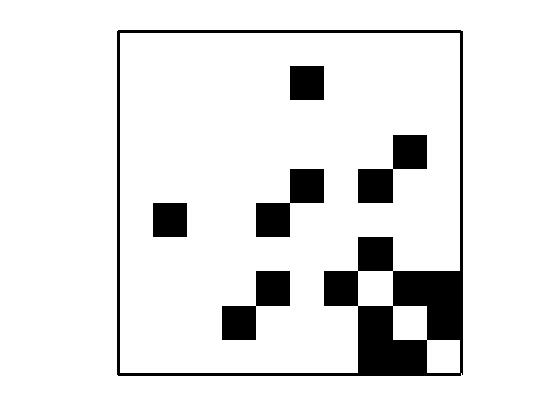
\includegraphics[width=0.225\textwidth]{\arraysfigsdir/adj.png}
      };
    \end{scope}
    \begin{scope}[xshift=0.08\textwidth]
      \node [mybox] (box){
        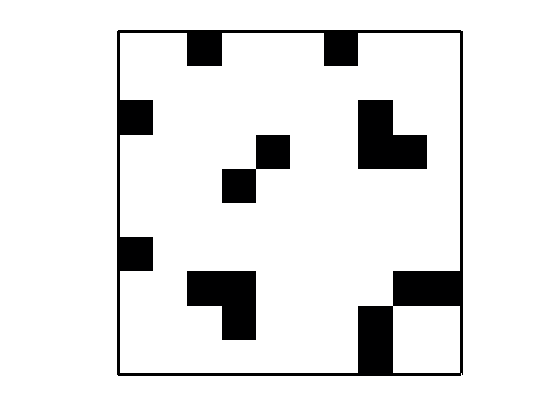
\includegraphics[width=0.225\textwidth]{\arraysfigsdir/adj_perm.png}
      };
    \end{scope}
    \begin{scope}[xshift=0.04\textwidth]
      \node[inner sep=0,text width=0.13\textwidth, text centered,font=\Huge] (note1) at (0,0) {
         $\equiv$};
    \end{scope}
  \end{scope}
\end{tikzpicture}

\end{tabular}
\caption[Illustration of array exchangeability for network adjacency matrices.]{Left: Networks with equivalent structure but different node labels. Right: Corresponding adjacency matrix representations of these networks}
\label{fig:networks:exchangeable}
\end{figure}

This symmetry weakens the hypothesis \eqref{eq:networks:exch} by demanding invariance only under a subset of all permutations of $\Nats^2$---those of the form $(i,j)\mapsto(p(i),p(j))$---we can no longer expect de Finetti's theorem to hold.
The relevant generalisation of the de Finetti theorem to this case is the following:
\begin{thm}[Aldous, Hoover]
  \label{theorem:ah}
  A random array $(\darray_{ij})$ is jointly exchangeable if and only if there is a random (measurable) function ${F:[0,1]^3\rightarrow\dataspace}$ such that the following holds: If $(\AHvar_i)_{i\in\Nats}$ and $(\AHvar_{\{ij\}})_{ij\in\Nats}$ are \iid sequences of ~$\Uniform[0,1]$ random variables, then
  \begin{equation}
    \label{eq:ah}
    (\darray_{ij})\eqdist (F(\AHvar_i,\AHvar_j,\AHvar_{\{ij\}})) \qquad\text{ for all }i,j\in\Nats\;.
  \end{equation}
\end{thm}

%\begin{rem}%\fTBD{To be reviewed. I have made reference to simplicity}
%\label{rem:U_ij}
%Note that the symmetry, $(U_{\{ij\}}) = (U_{\{ji\}})$ is not restrictive, in the sense that a representation where instead we had \eg $U_{ij}$ and $U_{ji}$ \iid is trivially jointly exchangeable and thus can be given a representation of the above form.
%\NA{In section \ref{sec:simple} we describe a representation result which does not involve $(U_{ij})$ and thus the symmetry does not place a restriction on potential models of $\darray$.}\fTBD{DR: Need to think about this.}
%\end{rem}
%\begin{rem}[symmetric arrays]\label{remsym}
%When modeling a symmetric array $X$, one can reduce the index set from ordered pairs $(i,j)$ to unordered pairs $\{i,j\}$.  
%In this case, $(X_{\{i,j\}}) \eqdist (F(U_i,U_j,U_{\{i,j\}}))$ where $F(\cdot,\cdot,d)$ is symmetric for every fixed value $d$.
%\end{rem}
\begin{rem}[separately exchangeable arrays]\label{remsep}
We say that an array $(X_{ij})$ is \emph{separately exchangeable} when $(X_{ij}) \eqdist (X_{p(i)p'(j)})$ for every pair $p,p' \in \SGinf$ of permutations. 
Such symmetry would be appropriate when modelling, e.g., a collaborative filtering task where the order of users and items are simultaneously irrelevant.
A separately exchangeable array can be seen to correspond with an off-diagonal subarray of a jointly exchangeable array, and thus can be shown to have the representation $(X_{ij}) \eqdist (F(U_i,V_j,W_{ij}))$, where $(U_i)$, $(V_j)$ and $(W_{ij})_{i,j\in\Nats}$ are \iid $\Uniform[0,1]$ random variables.
\end{rem}

%\subsection{Random graphs}

%The graph-valued data case $\dataspace=\lbrace{0,1}\rbrace$ is of particular interest. Here, the array $\darray$, interpreted as 
%an adjacency matrix, specifies a random simple graph with vertex set $\Nats$. If $\darray$ is symmetric, the graph is undirected. We call a 
%random graph exchangeable if $\darray$ satisfies \eqref{eq:jointly:ex}, \ie if its distribution is invariant under permutation of vertices.

%For undirected graphs, the representation \eqref{eq:ah} simplifies further:
%For any exchangeable undirected random graph, there is a random
%function ${\AHfunction:[0,1]^2\rightarrow[0,1]}$, symmetric in its arguments, such that
%\begin{equation}
%  \label{eq:ah:graphon:case}
  %(\darray_{ij})\eqdist 
%  F(\AHvar_i,\AHvar_j,\AHvar_{\{ij\}}):=\mathbb{I}\lbrace \AHvar_{\{ij\}} < \AHfunction(\AHvar_i,\AHvar_j)\rbrace\;.
%\end{equation}
%Each variable $\AHvar_i$ is associated with a vertex, each variable $\AHvar_{\{ij\}}$ with an edge. 
%The representation \eqref{eq:ah:graphon:case} is equivalent to the sampling scheme
%\begin{equation}
%  \label{eq:W:graph}
%  \AHvar_1,\AHvar_2,\dots\probgetsiid\Uniform[0,1]\qquad\text{and}\qquad X_{i,j}\probgets\Bernoulli(\AHfunction(\AHvar_i,\AHvar_j))\;,
%\end{equation}
%which is illustrated in figure~\ref{fig:W:graph}.
%If the graph is undirected, edges are sampled only for unordered index pairs as $\AHvar_{\lbrace ij\rbrace}$,
%and it is sufficient to consider symmetric functions $\AHfunction$.

%Recent work in discrete analysis shows that any measurable function $[0,1]^2\rightarrow[0,1]$ can be regarded as a (suitably defined) limit of adjacency matrices of graphs of increasing size \citep{Lovasz2006-hc}---intuitively speaking, 
%as the number of rows and columns increases, the
%matrix in figure~\ref{fig:W:graph} (right) converges to the heat map in figure~\ref{fig:W:graph} (middle).
%The figure also illustrates that convergence, and hence the parametrisation of the random graph distribution
%by $\AHfunction$, are only unique up to a reordering of rows and columns.

%In particular, if we fix an instance ${\AHfunction=\theta_0}$ and generate a random graph according to \eqref{eq:W:graph},
%we asymptotically recover the function $\theta_0$. This can be regarded as analogous to the law of large
%numbers, guaranteeing that a distribution can asymptotically be recovered from a sample.

\subsection{The general case: $d$-arrays}

Theorem \ref{theorem:ah} can in fact be stated in a more general setting than matrices, namely for random $d$-arrays, which are collections
of random variables of the form $(\{\darray_{i_1\dots i_d} : i_1,\dots,i_d\in\Nats\})$.
In particular, a sequence is a $1$-array, a matrix a $2$-array. A $d$-array 
can be interpreted as an encoding of a relation between $d$-tuples.
In this general case, theorem \ref{theorem:ah} still holds, but the random function $F$ in \eqref{eq:ah} is in general more complex:
In addition to the collections $(\AHvar_{i})$ and $(\AHvar_{\lbrace ij\rbrace})$ of uniform variables, the representation requires all
collections $(\AHvar_{\lbrace i_j\rbrace_{j\in I}})$ for any non-empty subset $I$ of the set $\lbrace 1,\ldots,d\rbrace$; \eg
$\AHvar_{\{i_1 i_3 i_4\}}$ for $d\geq 4$ and ${I=\lbrace 1,3,4\rbrace}$. The representation \eqref{eq:ah} is then substituted by
\begin{equation}
  F:[0,1]^{2^d-1}\to\dataspace\qquad\text{and}\qquad \darray_{i_1,\dots,i_d}=F(\AHvar_{I_1},\dots,\AHvar_{I_{(2^d-1)}})\;.
\end{equation}
For $d=1$, we recover de Finetti's theorem. In particular, if $\dataspace=\mathbb{R}$, $F$ is given by the inverse cumulative distribution function
of the random measure guaranteed by de Finetti's theorem.
%For a discussion of convergence properties of general arrays similar to those sketched above for random graphs, see \citep{Aldous2010-iw}.

Since we do not explicitly consider the case $d>2$ in our experiments in this chapter, we restrict 
our presentation throughout to the matrix-valued case for simplicity.
We note, however, that the model and inference algorithms described in the following are applicable to general array-valued data.
In chapter \ref{ch:arrays} we extend these representation results to arbitrary collections of arrays of arbitrary shape.

\section{A nonparametric model of exchangeable arrays}
\label{sec:networks:model}

To define a probabilistic model for array or graph valued data, we start with theorem \ref{theorem:ah}: A distribution on exchangeable matrices
can be specified by specifying a distribution on measurable functions $F : [0,1]^3\to\dataspace$.
For simplicity we restrict attention to symmetric matrices $X_{ij} = X_{ji}$; in chapter~\ref{ch:arrays} we present different arguments for which asymmetry is more elegantly handled but arrive at the same form of model.
We decompose the function $F$ into two functions 
${\AHfunction:[0,1]^2\rightarrow\latentspace}$ 
and ${H:[0,1]\times\latentspace\rightarrow\dataspace}$ for a suitable space $\latentspace$, such that
\begin{equation}
  \label{eq:decomposition}
  F(\AHvar_i,\AHvar_j,\AHvar_{\{ij\}})=H(\AHvar_{\{ij\}},\AHfunction(\AHvar_i,\AHvar_j))\;.
\end{equation}
Such a decomposition always exists---trivially, choose $\latentspace=[0,1]^2$.
Equivalently, there is a conditional probability $P[\,.\,|\AHfunction]$ on $\dataspace$ such that
\begin{equation}
  \label{eq:decomposition:sampling}
  F(\AHvar_i,\AHvar_j,\AHvar_{\{ij\}})\sim P[\,.\,|\AHfunction(\AHvar_i,\AHvar_j)]\;.
\end{equation}
Thus, \eqref{eq:decomposition} can be interpreted as a decomposition into a variable $\AHfunction$---the model parameter---which captures the structure of the underlying graph or array,
and random noise represented by $H$ or $P$, respectively.

To define a model, we assume $\AHfunction$ to be continuous, and to be distributed according to a Gaussian process. More precisely,
we set ${\latentspace = \Reals}$ and consider a zero-mean Gaussian process on 
$\cfspace_{\latentspace}:=\cfspace([0,1]^2,\latentspace)$, the space of continuous functions $[0,1]^2\rightarrow\latentspace$,
with kernel function 
${\kernel:[0,1]^2\times[0,1]^2\rightarrow\latentspace}$.
We assume the following generative model\footnotemark:
\begin{equation}
  \label{eq:model}
  \begin{split}
    \AHfunction\; &\probgets\; \gp{}(0,\kernel) \\
    \AHvar_{1},\AHvar_{2},\ldots\; &\probgetsiid\; \Uniform[0,1] \\
    \darray_{ij}\; &\probgets\; \likelihood[\,.\,|\AHfunction(U_i,U_j)] \;.
  \end{split}
\end{equation}
Additionally, the kernel may depend on parameters, which we denote by $\covhyppar$.
Since we have assumed $X$ to be symmetric we can ignore the potentially unusual depedencies introduced by $U_{\{ij\}}$ \eg we can restrict the model to the upper triangle of $X$.

The decomposition of $F$ introduces a natural set of latent variables $W_{ij}:=\AHfunction(\AHvar_i,\AHvar_j)$, conditioned on which the data is explained as $\darray_{ij}\sim\likelihood[\,.\,|\larray_{ij}]$. 
The parameter space of the model is the infinite-dimensional space $\cfspace_{\latentspace}$.
%Hence, the model is nonparametric.

The choice of $P$ depends on the type of data considered, two common cases are graphs and 
real-valued matrices.
In either case, the model first generates a latent matrix $W=(W_{ij})$. 
Depending on the type of data, observations could then be generated as follows:
\begin{center}
  \begin{tabular}{llll} 
    Observed data & Sample space & $P[\darray_{ij}\in\,.\,|\larray_{ij}]$  \\
    \midrule
    Graph & $\dataspace=\lbrace{0,1}\rbrace$  & $\Bernoulli(\logistic(\larray_{ij}))$
    \vspace{2pt}\\
    Real matrix & $\dataspace=\mathbb{R}$  & $\mbox{Normal}(\larray_{ij},\sigma_\dataspace^2)$\\
  \end{tabular}
\end{center}
where $\logistic$ is the logistic function, and $\sigma_\dataspace^2$ is a noise variance parameter.

The modelling assumptions we impose in addition to exchangeability are thus (i) that the function $\AHfunction$ is continuous---which implies measurability but is a stronger requirement---and (ii) that it is distributed according to a Gaussian process measure on $\cfspace_{\latentspace}$.
Additionally, (iii) the specific choice of $P$ may or may not introduce an additional assumption.
In the case of graphs, the only assumptions are (i) and (ii), the Bernoulli likelihood can be shown to be general \citep[e.g.][]{Aldous2010-iw}.
In the case of real-valued matrices, however, the model additionally assumes that the function 
$H$ in \eqref{eq:decomposition} is of the form
\begin{equation}
  H(\AHvar_{\{ij\}},\AHfunction(\AHvar_i,\AHvar_j))\eqdist \AHfunction(\AHvar_i,\AHvar_j)+\varepsilon_{\{ij\}} \qquad\text{ where }\qquad \varepsilon_{\{ij\}}\sim\mbox{Normal}(0,\sigma^2)\;.
\end{equation}

The Gaussian process prior favours smooth functions, which may result in interpretable latent space embeddings.
Inference in Gaussian processes is a well-understood problem, and the choice of a Gaussian prior allows us to leverage the full range of inference methods available for these models.

The model described in equation~\ref{eq:model} is illustrated for the case of graph data in figure~\ref{fig:networks:graphon}.
This demonstrates that $\Theta$ can be interpreted as a blurred adjacency matrix.

\begin{figure}[ht]
\centering
\begin{tabular}{c}
\begin{tikzpicture}[>=stealth,scale=0.0075\columnwidth]%,transform canvas={xshift=-3cm,yshift=1cm}]
  \begin{scope}[yshift=0.5cm]
  \begin{scope}
    \node [mybox] (box) at (0.5, -0.5){
    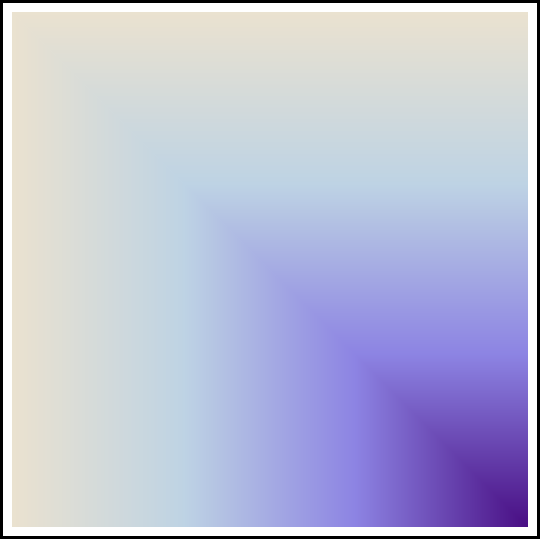
\includegraphics[width=0.225\columnwidth]{\arraysfigsdir/min_function.pdf} 
    };
    %\path[use as bounding box] (-0.5,0.5) rectangle (2.8,-1.5);
    %\draw (0,0) --(0,-1) --(1,-1) --(1,0) --(0,0);
    %\draw (0,0)--(1,-1);
    \node[font=\normalsize] at (0,0.1) {$0$};
    \node[font=\normalsize] at (-0.1,0) {$0$};
    \node[font=\normalsize] at (1,-1.1) {$1$};
    \node[font=\normalsize] at (1.1,-1) {$1$};
    \draw [dashed] (0.2,0.1) -- (0.2,-1.1); \node at (0.2,0.2) {$U_1$};
    \draw [dashed] (-0.1,-0.2) -- (1.1,-0.2); \node at (-0.25,-0.2) {$U_1$};
    \draw [dashed] (0.65,0.1) -- (0.65,-1.1); \node at (0.65,0.2) {$U_2$};
    \draw [dashed] (-0.1,-0.65) -- (1.1,-0.65); \node at (-0.25,-0.65) {$U_2$};
    \node[circle,fill,scale=0.4,color=red] at (0.65,-0.2) {};
  \end{scope}
  \begin{scope}[xshift=2cm]
    \draw (0,0)--(0,-1);
    \draw (-0.05,0)--(0.05,0); \node at (0.15,0) {$0$};
    \draw (-0.05,-1)--(0.05,-1); \node at (0.15,-1) {$1$};
    \node[circle,fill,scale=0.4,color=red] at (0,-0.21) {};
    \node[font=\normalsize] at (0.45,-0.23) {$\mbox{Pr}\lbrace X_{12}=1\rbrace$};
  \end{scope}
  \begin{scope}
  \draw[->] (0.7,-0.25) .. controls (1.3,-0.5) and (1.5,-0.5) .. (1.95,-0.26);
  \draw (1.4,-0.45) node [fill=white] {$\sigma(\Theta)$};
  \end{scope}
  \end{scope}
  %\begin{scope}[xshift=3.4cm]
  %  \node [mybox] (box){
  %  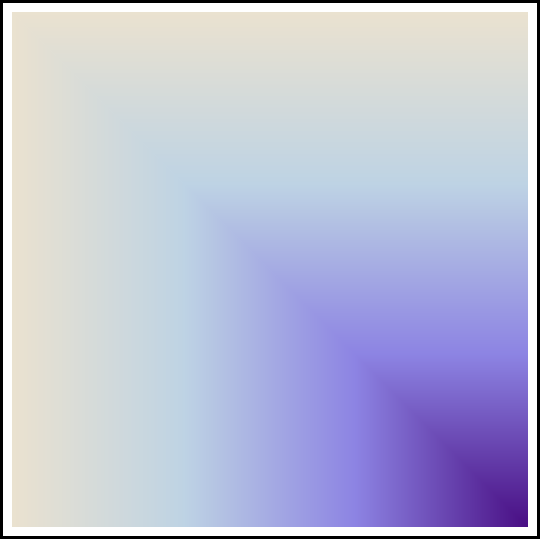
\includegraphics[width=0.18\columnwidth]{\arraysfigsdir/min_function.pdf} 
    %\includegraphics[width=2.9cm]{\arraysfigsdir/uniform_attachment_graphon.pdf}
  %};
  %\end{scope}  
  %\begin{scope}[xshift=3.4cm]
  \begin{scope}[xshift=-1.2cm]
    \node [mybox] (box){
    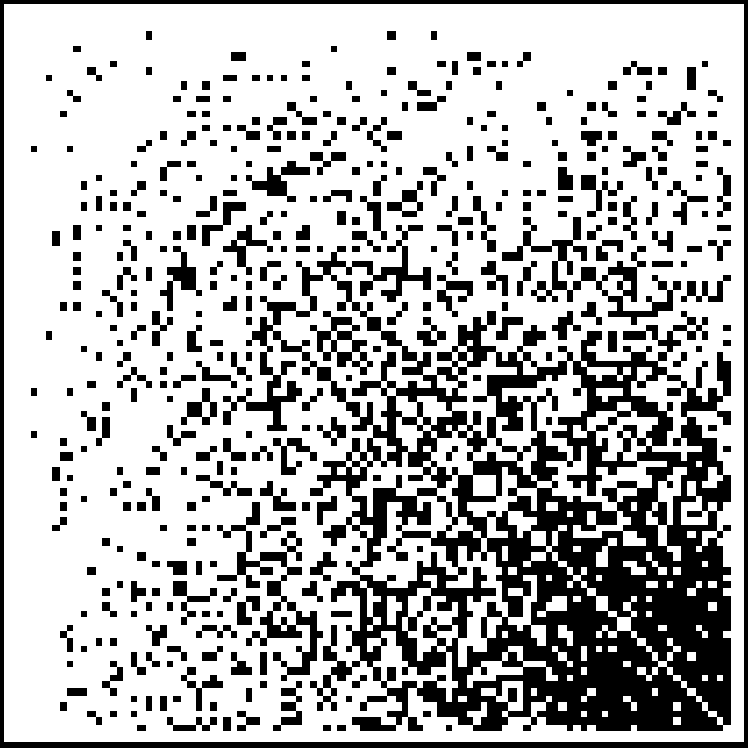
\includegraphics[width=0.225\columnwidth]{\arraysfigsdir/lovasz_sample100.pdf}
    %\includegraphics[width=2.8cm]{\arraysfigsdir/uniform_attachment_empirical.pdf}
  };
  \end{scope}
\end{tikzpicture}

\end{tabular}
\caption[Illustration of the Aldous--Hoover representation of a network.]{
Illustration of a model for network data inspired by the Aldous--Hover representation theorem.
The left shows a random sample of a binary network (represented by an adjacency matrix) generated by a model of the form given by equation~\eqref{eq:model}.
}
\label{fig:networks:graphon}
\end{figure}

\begin{rem}[Dense vs. sparse data]
  The methods described here address random matrices that are \emph{dense}, \ie as the size of a finite, observed $n\times n$ matrix increases,
  the number of non-zero entries (or the number of edges in a graph) grows as $O(n^2)$. Although the Aldous-Hoover theorem is sometimes invoked
  for data such as social networks, it should be kept in mind that network data is typically \emph{sparse}, with $O(n)$ non-vanishing entries.
  Density is an immediate consequence of theorem \ref{theorem:ah}: For graph data, for example, the asymptotic proportion of present edges is
  ${p:=\int\AHfunction(x,y)dxdy}$, and the graph is hence either empty (for $p=0$) or dense (since
  $O(pn^2)=O(n^2)$). Analogous representation theorems for sparse random graphs are to date an open problem in probability.
  There is however an emerging literature on representation theorems for sparse graphs including graphings \citep[e.g.][]{Lovasz2012-df}, thinning of graphon representations \citep{Wolfe2013-vs} and constructing graphs from exchangeable measures on $\mathbb{R}_+^2$ \citep{Caron2014-on}.
\end{rem}

\section{Related work}
\label{sec:networks:related}

Our model has some noteworthy relations to the Gaussian process latent variable model (GPLVM); a dimensionality-reduction technique \citep[e.g.][]{Lawrence2005-cn}.
GPLVMs can be applied to relational data \citep{Lawrence2009-za}, but doing so makes the assumption that either the rows or the columns of the random matrix are independent. 
In terms of our model, this corresponds to choosing kernels of the form $\kernel_\AHvar \otimes \delta_\AHvaralt$, where $\otimes$ represents the Kronecker matrix product and $\delta$ represents an `identity' kernel (\ie the corresponding kernel matrix is the identity matrix).
From this perspective, the application of our model to separately exchangeable real-valued matrices can be interpreted as a form of co-dimensionality reduction. 

A related parametric model is the eigenmodel of \citet{Hoff2007-ja}.
This model, also justified by exchangeability arguments, approximates a matrix with a bilinear form, followed by some link function and distribution depending on the type of data.
We show in proposition \ref{prop:matrixfactorisation} that this can be represented in the form of our model by using a kernel function of the form $L_\AHvar \otimes L_\AHvaralt$ where $L$ represents the dot product kernel (\ie the kernel that gives rise to linear functions).

%\fTBD{To be reviewed - also mentions nonparametric matrix factorisation}
Available models for graph data include the parametric mixed membership stochastic blockmodel (MMSB; \cite{Airoldi2008-fr}) and nonparametric infinite relational model (IRM; \cite{Kemp2006-jt}), latent feature relational model (LFRM; \cite{Miller2009-wg}), infinite latent attribute model (ILA; \cite{Palla2012-ch}) and many others.
%\NA{
Similar models also exist for real valued matrices, including the infinite hidden relational model (IHRM; \cite{Xu2006-uy}) which is a counterpart to the IRM and binary matrix factorisation (BMF; \cite{Meeds2007-gd}) which is a counterpart to the LFRM.
%}

\citet{Roy2009-ge} present a nonparametric Bayesian model of relational data that approximates $\AHfunction$ by a piece-wise constant function whose hierarchical structure is a Mondrian process. In contrast, we approximate $\AHfunction$ by a smooth function.

A recent development is the Sparse Matrix Variate Gaussian Process Blockmodel (SMGB; \cite{Yan2011-lc}), and the extension to higher order arrays (InfTucker; \cite{Xu2012-ub}).
Although not motivated in terms of exchangeability, these Gaussian process models do not impose independence assumptions on either rows or columns, in contrast to the GPLVM.
These models can be represented as placing a prior ${\AHfunction \dist \GP\,(0, \kernel_1 \otimes \kernel_2)}$ on the function $\AHfunction$ in \eqref{eq:decomposition}.
%\fTBD{Needs review}
This prior is equivalent to \eqref{eq:model} for some common choices of kernel $\kernel$ (\eg squared exponential) but excludes others such as those that give rise to symmetric functions or additive kernels.
Existing efficient algorithms for Gaussian processes of this form \citep[e.g.][]{Saatci2011-yo} perform calculations using a complete grid of data, which results in computational complexities that depend on the size of the array.
Our work suggests that it may not be necessary to impose Kronecker product structure on the kernel, which allows for inference with improved scaling when data is sparsely observed.
However, their most recent work \citep{Zhe2013-tv} has employed many other approximate inference strategies resulting in an algorithm that can be applied to data much larger than that considered here.

\subsection{A common perspective on the literature}

The representations \eqref{eq:decomposition} and \eqref{eq:decomposition:sampling} allow for a common perspective on a range of models in the literature depending on how they construct $(W_{ij})$ or place a prior over $\AHfunction$.
The following proposition allows us to specify many models in both forms.
%In fact, one can show an equivalence between these different ways of specifying a model as described in the following proposition which is a trivial extension of a similar result linking linear regression and Gaussian process regression \cite[Bishop book?].

\begin{prop}
\label{prop:matrixfactorisation}
A matrix factorisation model defined as
\begin{equation}
W_{ij} = \AHvar_i\Lambda\AHvaralt_j' \quad \quad \Lambda_{ij} \simiid \Normal (0, 1)
\end{equation}
is equivalent to
\begin{equation}
W_{ij} = \AHfunction\,(\AHvar_i, \AHvaralt_j) \quad \quad \AHfunction \sim \GP\,(0, L_\AHvar \otimes L_\AHvaralt)
\end{equation}
where $L_U(\AHvar_{i_1}, \AHvar_{i_2}) = \AHvar_{i_1}\AHvar_{i_2}'$ and similarly for $L_V$.
\end{prop}

\begin{proof}
For a finite collection of $(W_{ij})$, the Gaussian process model can be written as
\begin{equation}
(W_{ij}) \sim \Normal\,(0, K_U \otimes K_V)
\end{equation}
where $K$ is the kernel matrix corresponding to the kernel function $L$ and $\otimes$ represents a Kronecker product.
In the matrix factorisation, $W_{ij}$ is a linear combination of Gaussian distributed random variables and hence is Gaussian distributed itself. Thus, we need only show that it has zero mean and the required covariance structure. This is trivial,
\begin{eqnarray}
\mathbb{E} (W_{ij} \given \AHvar_i, \AHvaralt_j) = \AHvar_i\mathbb{E}(\Lambda)\AHvaralt_j' & = & 0 \\
\textrm{Cov} (W_{i_1j_1}, W_{i_2j_2} \given \AHvar_{i_1}, \AHvar_{i_2}, \AHvaralt_{j_1}, \AHvaralt_{j_2}) & = & \mathbb{E} (W_{i_1j_1} W_{i_2j_2} \given \AHvar_{i_1}, \AHvar_{i_2}, \AHvaralt_{j_1}, \AHvaralt_{j_2} ) \nonumber \\
%& = & \mathbb{E}\bigg(\Big(\sum_{k_1,l_1} u_{i_1k_1}v_{j_1l_1}\lambda_{k_1,l_1}\Big)\Big(\sum_{k_2,l_2} u_{i_2k_2}v_{j_2l_2}\lambda_{k_2l_2}\Big)\bigg) \nonumber \\
& = & \sum_{k_1,l_1,k_2,l_2} u_{i_1k_1}v_{j_1l_1}u_{i_2k_2}v_{j_2l_2}\mathbb{E}(\lambda_{k_1,l_1}\lambda_{k_2l_2}) \nonumber \\
& = & \Big(\sum_k u_{i_1k}u_{i_2k}\Big)\Big(\sum_l v_{j_1l}v_{j_2l}\Big) \nonumber \\
& = & \AHvar_{i_1}\AHvar_{i_2}' \times \AHvaralt_{j_1}\AHvaralt_{j_2}'.
\end{eqnarray}
\end{proof}

This correspondence between matrix factorisation and priors on functions can be kernelized by mapping $\AHvar_i, \AHvaralt_j$ through functions $\phi_U, \phi_V$ respectively.
Thus, we see that a Gaussian process model using a tensor product of general kernels is equivalent to kernelized matrix factorisation.

This correspondence allows us to succinctly summarise many of the models in the literature review in table \ref{table:ModelComparison} below (the model introduced here is referred to as the random function model).

\begin{table}[h]
  \centering
  \begin{tabular}{l|ccc}%c} 
%    \toprule
    & $W_{ij}$ & $\kernel$ & $U_i, V_j \in \, .$ \\% & $\dataspace$\\ 
    %\multicolumn{4}{c}{Graph data}\\
    \midrule
    %\addlinespace[2pt]
    %\textcolor{red}{Random function model} 
    Random function model & $\phi(U_i, V_j)\Lambda$ & $\kernel_{U\times V}$ & $\Reals^d \, , \, [0,1]$\\% & All\\
    SMGB, InfTucker & $\phi(\AHvar_i)'\Lambda\phi(\AHvaralt_j)$ & $\kernel_U \otimes \kernel_V$ & $\Reals^d$\\% & $\{0,1\},\, \Reals$\\
    GPLVM, Kernel PCA & $\phi(\AHvar_i)\Lambda$ & $\kernel_\AHvar \otimes \delta_V$ & $\Reals^d$ \\% & All\\
    Eigenmodel & $\AHvar_i\Lambda \AHvaralt_j'$ & $L_U \otimes L_V$ & $\Reals^d$ \\% & All\\
    Linear relational GP & $\AHvar_i\Lambda \AHvaralt_j'$ & $L_U \otimes L_V$ & $\Reals^d$ \\% & $\{0,1\}$\\
    PMF & $\AHvar_i V_j'$ & 0 & $\Reals^d$ \\% & $\Reals$\\
    PCA, Factor analysis, etc. & $\AHvar_i\Lambda$ & $L_U \otimes \delta_V$ & $\Reals^d$ \\% & $\Reals$\\
    Latent distance & $-|\AHvar_i - \AHvar_j|$ & 0 & $\Reals^d$ \\% & $\{0,1\}$\\
    Mondrian process based & Decision tree & * & $[0, 1]^d$ \\% & All\\
    \midrule
    Latent class & $\Lambda_{\AHvar_i\AHvar_j}$ & $\delta_{U\times U}$ & $\{1,\ldots,d\}$ \\% & $\{0,1\}$\\
    IRM &$\Lambda_{\AHvar_i\AHvar_j}$ & $\delta_{U\times U}$ & $\{1,\ldots,\infty\}$ \\% & $\{0,1\}$\\
    IHRM  &$\Lambda_{\AHvar_i\AHvaralt_j}$ & $\delta_{U\times V}$ & $\{1,\ldots,\infty\}$ \\% & $\Reals$\\
    BMF  & $\AHvar_i\Lambda \AHvaralt_j'$ & $L_U \otimes L_V$ & $\{0,1\}^\infty$ \\% & $\Reals$\\
    LFRM  & $\AHvar_i\Lambda \AHvar_j'$ & $L_U \otimes L_U$ & $\{0,1\}^\infty$ \\% & $\{0,1\}$\\
    ILA & $\sum_d \mathbb{I}_{U_{id}}\mathbb{I}_{U_{jd}}\Lambda^{(d)}_{U_{id}U_{jd}}$ & * & $\{0,\ldots,\infty\}^\infty$ \\% &$\{0,1\}$ \\
    %\midrule
    %\addlinespace[4pt]
    %\multicolumn{4}{c}{Real-valued matrix data}\\
    %\midrule
    %\textcolor{red}{Random function model} 
%\bottomrule
\end{tabular}
\caption[Summary of models of arrays cast into Aldous--Hoover form.]{
Summary of models classified by equation for $W_{ij}$, equivalent kernel $\kernel$ in GP representation and domain of latent variables $(U_i), (V_j)$.
$\Lambda$ is a matrix $\phi$ is some mapping into a feature space and $\mathbb{I}_A$ is the indicator function of the event $A>0$.
$\kernel$ represents any kernel function, $\delta$ the identity kernel function, $L$ the simple dot product kernel function and $L^k$ is the dot product kernel applied only to the $k$th components of its arguments.
}
\label{table:ModelComparison}
\end{table}

Table~\ref{table:ModelComparison} necessarily glosses over many details (\eg choice of priors, inference methods), but it is hoped that it reveals the structural similarities between many models in the literature.
Despite not often being viewed as a network model we have included principal component analysis (PCA) as a linear counterpart to the non-linear GPLVM.

This table reveals that the majority of models included here model $\AHfunction$ as linear or bilinear (potentially kernelized).
The Mondrian process based model \citep{Roy2009-ge} is a notable exception since it models $\AHfunction$ as a piecewise constant random function which is fundamentally different from our approach of modelling $\AHfunction$ to be continuous.
For simplicity we have refrained from writing down the kernel corresponding to the Mondrian process based model; it could be described as an indicator function of the equivalence class induced by the Mondrian process.
We also see that the ILA model is significantly more flexible in its specification of $\AHfunction$ than other models using discrete latent variables.
Again, we refrain from writing down what would be a fairly complicated kernel function corresponding to this model.

%This table could be interpreted as revealing that our model is a small modification of other models that use latent variables in $\Reals^d$.
%However, we would argue that our work is a joint generalisation rather than a modification.
%Despite being more general, our model is arguably simpler and firmly rooted in the relevant theory (and achieves good empirical performance as shown in section \ref{sec:experiments}).

We note that the nonparametric Gaussian process prior on $\AHfunction$ in the random function models means that, if supported by the data, the posterior distribution of $\AHfunction$ could approximate any of the functions specified by other models.
This is of course true of the other nonparametric models; particular priors will influence the rate at which different forms of $\AHfunction$ can be inferred.

\section{Posterior computation}
\label{sec:Inference}

In this section we describe Markov Chain Monte Carlo (MCMC) algorithms for generating approximate samples from the posterior distribution of the model parameters given a partially observed array.  Most importantly, we describe a random subset-of-regressors approximation that scales to graphs with hundreds of nodes and tens of thousands of edge observations. Given the relatively straightforward nature of the proposed algorithms and approximations, we refer the reader to other papers whenever appropriate.

\subsection{Latent space and kernel}
\label{sec:Kernel}
The random function representation in theorem \ref{theorem:ah} is not restricted to the use of uniform distributions for the variables $(\AHvar_i)$.
The uniform distributions arise in the proof of the theorem as generic distributions with which one can encode the information of other random variables via a measurable function.
Therefore, the proof remains unchanged if one replaces the uniform distributions with any isomorphic probability distribution \ie any non-atomic
probability measure on a Borel space.
For the presentation in section~\ref{sec:background}, the domain $[0,1]^2$ of the pairs of uniforms provides an intuitive analogy
with adjacency matrices.
For the purposes of inference, normal distributions are more convenient, and we henceforth use ${\AHvar_{1},\AHvar_{2},\ldots\; \simiid \Normal(0, I_r)}$ for some integer $r$.

Since we focus on undirected graphical data, we require the symmetry condition $\larray_{ij} = \larray_{ji}$. This can be achieved by constructing the kernel function in the following way \citep[e.g.][]{Duvenaud2014-em}
\begin{eqnarray}
\kernel(\inputpoints_1, \inputpoints_2) & = & \frac{1}{2}\big(\bar\kernel(\inputpoints_1, \inputpoints_2) + \bar\kernel(\inputpoints_1, \bar\inputpoints_2)\big) + \sigma^2I \quad \quad \textrm{(Symmetry + noise)} \\
\bar\kernel(\inputpoints_1, \inputpoints_2) & = & \scalefactor^2\exp(-|\inputpoints_1 - \inputpoints_2|^2/(2\lengthscale^2)) \quad \quad \quad \quad \quad \textrm{(RBF kernel)}
\end{eqnarray}
where $\inputpoints_k = (\AHvar_{i_k}, \AHvar_{j_k})$, $\bar\inputpoints_k= (\AHvar_{j_k}, \AHvar_{i_k})$ and $\scalefactor, \lengthscale, \sigma$ represent a scale factor, length scale and noise respectively (see \eg chapter~\ref{ch:construction}). We collectively denote the kernel parameters by $\covhyppar$.
For undirected data one can model only the upper triangular part of the adjacency matrix.

\subsection{Sampling without approximating the model}

\newcommand{\numobs}{\mathrm O}
\newcommand{\numnodes}{\mathrm N}
In the simpler case of a real-valued array $\darray$, we construct an MCMC algorithm over the variables $((\AHvar_i),\covhyppar, \sigma_\darray)$ by repeatedly slice sampling \citep{Neal2003-zv} from the conditional distributions
\[
\covhyppar_i \given \covhyppar_{-i}, \sigma_\darray, (\AHvar_i), \darray
\qquad\quad
\sigma_\darray \given \covhyppar, (\AHvar_i), \darray
\qquad\quad \text{and} \qquad\quad
\AHvar_j \given \AHvar_{-j}, \covhyppar, \sigma_\darray, \darray
\]
where $\sigma_\darray$ is the noise variance parameter used when modelling real valued data introduced in section \ref{sec:networks:model}.
Let $\numnodes = |(\AHvar_{i})|$ denote the number of rows in the observed array,
let $\inputpoints$ be the set of all pairs $(\AHvar_i,\AHvar_j)$ for all observed relations $\darray_{ij}$, 
let $\numobs = |\inputpoints|$ denote the number of observed relations,
and 
let $K$ represent the $\numobs \times \numobs$ kernel matrix between all points in $\inputpoints$. Changes to $\covhyppar$ affect every entry in the kernel matrix $K$ and so, naively, the computation of the Gaussian likelihood of $\darray$ takes $\CompOrder(\numobs^3)$ time.  Likewise, changes to $(\AHvar_i)$ also affect entries in $K$. Naively re-evaluating the Gaussian likelihood term again takes $\CompOrder(\numobs^3)$ time, and so, across all $\numnodes$ rows, we expend $\CompOrder(\numobs^3 \numnodes)$ time. Whether or not this can be improved by exploiting structure in the modifications, the cubic dependence on $\numobs$ seems unavoidable, and thus this naive algorithm is unusable for all but very small data sets. 


\subsection{A random subset-of-regressor approximation}

In order to scale the method to much larger graphs, we applied a variation of a sparse approximation method known as Subsets-of-Regressors, or simply SoR \citep{Alex_J_Smola2001-ev,Wahba1999-bl,Silverman1985-ys} (See \citet{Quinonero-Candela2005-er} for an excellent survey of this and other sparse approximations).
The SoR approximation replaces the infinite dimensional GP with a finite dimensional approximation.
Our approach is to treat both the inputs and outputs of the GP as latent variables.
%, a random version of the SoR approximation appears to work very well, even with few pseudoinputs (see below).

In particular, 
introduce $k$ Gaussian distributed pseudoinputs $\pseudopoints=(\pseudopoints_1,\dotsc,\pseudopoints_k)$, and, for each $j=1,\dotsc,k$, define target values ${\targets_j = \AHfunction(\pseudopoints_j)}$.  In other words, writing $K_{\pseudopoints\pseudopoints}$ for the kernel matrix formed from the pseudoinputs $\pseudopoints$, we have
\[
(\pseudopoints_i) \simiid \Normal(0,1) \qquad\text{and}\qquad
\targets \given \pseudopoints \sim \Normal(0,K_{\pseudopoints\pseudopoints}).
\]
The idea of the SoR approximation is to replace $\larray_{ij}$ with the posterior mean conditioned on $(\pseudopoints,\targets)$,
\[
\larray = K_{\inputpoints\pseudopoints} K_{\pseudopoints\pseudopoints}^{-1}\targets,
\label{eqn:GPConditional}
\]
where $K_{\inputpoints\pseudopoints}$ is the kernel matrix between the latent embeddings $\inputpoints$ and the pseudoinputs $\pseudopoints$.  By considering random pseudoinputs, we construct an MCMC analogue of the techniques proposed in~\cite{Titsias2008-gp}.
% in be seen to be doing a Bayesian version of sparse variational techniques proposed by Titsias and Lawrence \cite{Titsias2010}.

Given this approximate model, the conditional distribution $\targets \given (\AHvar_i), \pseudopoints, \covhyppar, (\sigma_\darray), \darray$ is amenable to elliptical slice sampling \citep{Murray2010-zu}, for both real valued and binary $\darray$. All other random parameters, including the $(U_i)$ and $(\eta_i)$, can again be sampled from their full conditional distributions using slice sampling.  The sampling algorithms require that one computes expressions involving~\eqref{eqn:GPConditional}. As a result they cost at most $\CompOrder(k^3 \numobs)$.

%These sampling algorithms now require that one recomputes at most $K_{\pseudopoints\pseudopoints}^{-1}$ (or more precisely the Cholesky decomposition) and $K_{\inputpoints\pseudopoints}^{-1}$.  As a result, they cost at most $\Theta(k^3 \numobs)$ time. 

\section{Experiments}
\label{sec:experiments}
We evaluate the model on three different network data sets (see table~\ref{table:networks:datasets}). Two of these data sets---the high school and NIPS co-authorship data---have been extensively
analysed in the literature.
The third data set, a protein interactome, was previously noted by \citet{Hoff2007-ja} to be of interest since it exhibits both block structure and transitivity.

\begin{table}
\begin{center}
  \begin{tabular}{l  l  c  l}
    Data set & Recorded data & Vertices & Reference\\
    \midrule
    High school & high school social network & 90 & e.g.\ \cite{Hoff2007-ja} \\
    NIPS & subset of coauthorship network & 234 & e.g.\ \cite{Miller2009-wg} \\
    Protein & protein interactome & 230 & e.g.\ \cite{Hoff2007-ja}
  \end{tabular}
\end{center}
  \caption[Summary of data sets in link prediction experiment.]{Summary of data sets in link prediction experiment.}
  \label{table:networks:datasets}
\end{table}

We compare performance of our model on these data sets to three other models (see table~\ref{table:networks:datasets}), probabilistic matrix factorization (PMF) \citep{Salakhutdinov2008-tp},
Hoff's eigenmodel \citep{Hoff2007-ja}, and the GPLVM \citep{Lawrence2005-cn}. The models are chosen for comparability, since they all embed nodes into a Euclidean latent space.
%All of these models represent nodes as being embedded in a latent space, although the approaches vary considerably.
Experiments for all three models were performed using reference implementations by the respective 
authors (see table~\ref{table:networks:algorithms} for additional algorithm details).\footnotemark

\footnotetext{Implementations are available for PMF at
\url{http://www.mit.edu/~rsalakhu/software.html};
for the eigenmodel at
http://cran.r-project.org/src/contrib/Descriptions/eigenmodel.html;
and for the GPLVM at
\url{http://www.cs.man.ac.uk/~neill/collab/}.}

\begin{table}
\begin{center}
  \begin{tabular}{l  l  c  l }
    Model & Method & Iterations [burn-in] & Parameters\\
    \midrule
    PMF & stochastic gradient & 1000 & author defaults
    \\
    Eigenmodel & MCMC & 10000 [250] & author defaults
    \\
    GPLVM & stochastic gradient  & 20 sweeps & author defaults
    \\
    Random function model & MCMC & 1000 [200] & (see below)
  \end{tabular}
  %\label{table:DataSets}
  %\end{table}
\end{center}
  \caption[Summary of algorithms and settings in link prediction experiment.]{Summary of algorithms and settings in link prediction experiment.}
  \label{table:networks:algorithms}
\end{table}

We use standard normal priors on the latent variables $\AHvar$ and pseudo points $\pseudopoints$, and log normal priors for kernel parameters.
\vspace{-0.18cm}
\parpic(7cm,3.9cm)[r]{
\begin{minipage}[h]{8cm}
%\begin{table}
\begin{center}
  \begin{tabular}{c | c c c}
    {} & exp mean & std & width \\
    \midrule
    length scale & 1 & 0.5 & 0.5 \\
    scale factor & 2 & 0.5 & 0.5 \\
    target noise & 0.1 & 0.5 & 0.1 \\
    $\AHvar$ & - & - & 4 \\
    $\pseudopoints$ & - & - & 2
  \end{tabular}
\end{center}
%  \caption[Parameter settings for the RFM.]{Parameter settings for the RFM.}
%  \label{table:networks:params}
%\end{table}
\end{minipage}}
Slice sampling parameters are chosen to favour slice sampling acceptance after a reasonable number of iterations, as evaluated over a range of data sets.
Specific values of prior and sampling parameters are summarised in the table on the right.
To balance the computational demands of the different sampling steps, we sampled $\targets$ 50 times per iteration whilst all other variables were sampled once per iteration.

In all experiments, we partitioned the edge data into 5 equally sized partitions and performed 5-fold cross validation, predicting the links in one held out partition given the other 4. 
Where the models did not restrict their outputs to values between 0 and 1, we truncated any predictions lying outside this range.
Tbale~\ref{table:networks:AUCs} reports average AUC (area under receiver operating characteristic) for the various models, with numbers for the top performing model set in bold.
Significance of results is evaluated by means of a $t$-test with a $p$-value of 0.05; results for models not distinguishable from the top performing model in terms of this $t$-test are also set in bold.

\begin{table}
\begin{center}
  \begin{tabular}{r | r r r | r r r | r r r}
    \multicolumn{10}{c}{AUC results} \\
    \addlinespace[2pt]
    Data set & \multicolumn{3}{c|}{High school} & \multicolumn{3}{c|}{NIPS} & \multicolumn{3}{c}{Protein} \\
    $d$ & 1 & 2 & 3 & 1 & 2 & 3 & 1 & 2 & 3 \\
    \midrule
    PMF                   & 0.747 & 0.792 & 0.792 & 0.729 & 0.789 & 0.820 & 0.787 & 0.810 & 0.841 \\
    Eigenmodel            & 0.742 & 0.806 & 0.806 & 0.789 & 0.818 & 0.845 & 0.805 & 0.866 & 0.882 \\
    GPLVM                 & 0.744 & 0.775 & 0.782 & 0.888 & 0.876 & 0.883 & 0.877 & 0.883 & 0.873 \\
    RFM & \textbf{0.815} & \textbf{0.827} & \textbf{0.820} & \textbf{0.907} & \textbf{0.914} & \textbf{0.919} & \textbf{0.903} & \textbf{0.910} & \textbf{0.912}
  \end{tabular}
\end{center}
  \caption[AUCs in link prediction experiment.]{Average AUC for each method and dataset. $d$ is the dimensionality of the latent variables used in each method. Results that are not distinguishable from the best performing method by a $t$-test at 5\% significance are set in bold.}
  \label{table:networks:AUCs}
\end{table}

%The random function model outperforms the other models in almost all tests.
The random function model outperforms the other models in \emph{all} tests.
%We also note that in most experiments, a single latent dimension suffices to achieve better performance, even when the other models use additional latent dimensions.
We also note that in all experiments, a single latent dimension suffices to achieve better performance, even when the other models use additional latent dimensions.
%\fTBD{Remove this sentence, if we just go with the new experiments}
%\NA{
%Since our first experiments, we investigated the single poor result observed on the High school data set (3 dimensions).
%The weak performance in this case was due to slow mixing of $\AHvar$ and $\pseudopoints$ as identified by Geweke tests \citep{Geweke2004}.
%We have subsequently found that sampling these variables on each iteration greatly improves mixing.
%We have shown the numerical results for this improved MCMC schedule in {\color{gray}\textit{gray italics}} to avoid mixing training and testing.
%With this more sensible MCMC schedule the random function model outperforms the other models across the board.
%}

In general, a more general model of data will not necessarily improve empirical performance compared to simpler models.
However, our results provide empirical evidence that the flexibility of a general nonparametric model can make an important difference for the problems considered here.

The posterior distribution of $\AHfunction$ favours functions defining random array distributions that explain the data well.
In this sense, our model fits a probability distribution.
The standard inference methods for GPLVM and PMF applied to relational data, in contrast, are designed to fit mean squared error, and should therefore be expected to show stronger performance under a mean squared error metric.
As table~\ref{table:networks:RMSEs} shows, this is indeed the case.
The reported values are RMSE results, with significance evaluated as above.

%\begin{center}
%  \begin{tabular}{r | r r r | r r r | r r r}
%    \multicolumn{10}{c}{RMSE results} \\
%    \addlinespace[2pt]
%    Data set & \multicolumn{3}{c|}{High school} & \multicolumn{3}{c|}{NIPS} & \multicolumn{3}{c}{Protein} \\
%    Latent dimensions & 1 & 2 & 3 & 1 & 2 & 3 & 1 & 2 & 3 \\
%    \midrule
%    PMF                   & 0.245 & 0.242 & 0.240 & 0.141 & 0.135 & 0.130 & 0.151 & 0.142 & 0.139 \\
%    Eigenmodel            & 0.244 & \textbf{0.238} & \textbf{0.236} & 0.141 & 0.132 & 0.124 & 0.149 & 0.142 & \textbf{0.138} \\
%    GPLVM                 &0.244 & 0.241 & 0.239 & \textbf{0.112} & \textbf{0.109} & \textbf{0.106} & \textbf{0.139} & \textbf{0.137} & \textbf{0.138} \\
%    RFM & \textbf{0.241} & \textbf{0.236} & 0.248 & 0.126 & \textbf{0.115} & \textbf{0.109} & 0.144 & 0.141 & 0.140 \\
%    \color{gray}
%    \textit{RFM} & \color{gray}\textit{0.239} & \color{gray}\textit{0.234} & \color{gray}\textit{0.235} & \color{gray}\textit{0.114} & \color{gray}\textit{0.111} & \color{gray}\textit{0.110} & \color{gray}\textit{0.138} & \color{gray}\textit{0.136} & \color{gray}\textit{0.136}
%  \end{tabular}
%\end{center}

\begin{table}
\begin{center}
  \begin{tabular}{r | r r r | r r r | r r r}
    \multicolumn{10}{c}{RMSE results} \\
    \addlinespace[2pt]
    Data set & \multicolumn{3}{c|}{High school} & \multicolumn{3}{c|}{NIPS} & \multicolumn{3}{c}{Protein} \\
    $d$ & 1 & 2 & 3 & 1 & 2 & 3 & 1 & 2 & 3 \\
    \midrule
    PMF                   & 0.245 & 0.242 & 0.240 & 0.141 & 0.135 & 0.130 & 0.151 & 0.142 & 0.139 \\
    Eigenmodel            & 0.244 & 0.238 & \textbf{0.236} & 0.141 & 0.132 & 0.124 & 0.149 & 0.142 & \textbf{0.138} \\
    GPLVM                 &0.244 & 0.241 & 0.239 & \textbf{0.112} & \textbf{0.109} & \textbf{0.106} & \textbf{0.139} & \textbf{0.137} & \textbf{0.138} \\
    RFM & \textbf{0.239} & \textbf{0.234} & \textbf{0.235} & \textbf{0.114} & \textbf{0.111} & \textbf{0.110} & \textbf{0.138} & \textbf{0.136} & \textbf{0.136}
  \end{tabular}
\end{center}
  \caption[RMSEs in link prediction experiment.]{Average RMSE for each method and dataset. $d$ is the dimensionality of the latent variables used in each method. Results that are not distinguishable from the best performing method by a $t$-test at 5\% significance are set in bold.}
  \label{table:networks:RMSEs}
\end{table}

An arguably more suitable metric is comparison in terms of conditional edge probability \ie ${\likelihood(\darray_{\lbrace ij \rbrace} \given \larray_{\lbrace ij \rbrace})}$ for all $i,j$ in the held out data. These cannot, however, be computed in a meaningful manner for
standard versions of models such as PMF and GPLVM, which assign a Gaussian likelihood to data. Table~\ref{table:networks:probs} hence reports only comparisons to the eigenmodel.
%This table is negative conditional log likelihood * 1000 / (number of predicted links).
%\begin{center}
%  \begin{tabular}{r | r r r | r r r | r r r}
%     \multicolumn{10}{c}{Negative log conditional edge probability\footnotemark} \\
%     \addlinespace[2pt]
%     Data set & \multicolumn{3}{c|}{High school} & \multicolumn{3}{c|}{NIPS} & \multicolumn{3}{c}{Protein} \\
%    Latent dimensions & 1 & 2 & 3 & 1 & 2 & 3 & 1 & 2 & 3 \\
%    \midrule
%    Eigenmodel & 220 & \textbf{210} & \textbf{200} & 88 & 81 & 75 & 96 & 92 & 86 \\
%    RFM        & \textbf{210} & \textbf{200} & 240 & \textbf{71} & \textbf{58} & \textbf{55} & \textbf{83} & \textbf{81} & \textbf{79}  \\
%    \color{gray}
%    \textit{RFM} & \color{gray}\textit{205} & \color{gray}\textit{199} & \color{gray}\textit{201} & \color{gray}\textit{65} & \color{gray}\textit{57} & \color{gray}\textit{56} & \color{gray}\textit{78} & \color{gray}\textit{75} & \color{gray}\textit{75}
%  \end{tabular}
%\end{center}

\begin{table}
\begin{center}
  \begin{tabular}{r | r r r | r r r | r r r}
     \multicolumn{10}{c}{Negative log conditional edge probability} \\
     \addlinespace[2pt]
     Data set & \multicolumn{3}{c|}{High school} & \multicolumn{3}{c|}{NIPS} & \multicolumn{3}{c}{Protein} \\
    $d$ & 1 & 2 & 3 & 1 & 2 & 3 & 1 & 2 & 3 \\
    \midrule
    Eigenmodel & 220 & 210 & \textbf{200} & 88 & 81 & 75 & 96 & 92 & 86 \\
    RFM & \textbf{205} & \textbf{199} & \textbf{201} & \textbf{65} & \textbf{57} & \textbf{56} & \textbf{78} & \textbf{75} & \textbf{75}
  \end{tabular}
\end{center}
  \caption[Negative log conditional edge probabilities in link prediction experiment.]{Average negative log conditional edge probability for the Eigenmodel and RFM and each dataset.
  The precise calculation implemented is $-\log(\likelihood(\darray_{\lbrace ij \rbrace} \given \larray_{\lbrace ij \rbrace})) \times 1000 \, / \,(\textrm{Number of held out edges})$.
  $d$ is the dimensionality of the latent variables used in each method. Results that are not distinguishable from the best performing method by a $t$-test at 5\% significance are set in bold.}
  \label{table:networks:probs}
\end{table}

\subsection{Inferred representing functions}

We now discuss what can be learned about a network by inspecting the posterior for the representing function $\Theta$.
Figure~\ref{fig:(R)GPLVM_Comparison} shows a visualisation of the protein interactome (left), its adjacency matrix (middle) and approximate maximum a posteriori (MAP) estimate of $\Theta$ (right).
The adjacency matrix has been sorted by the values of the approximate MAP $(U_i)$.

\begin{figure}[ht]
  \centering
  \begin{tikzpicture}%[transform canvas={xshift=-1cm,yshift=0cm}]
  %\path[use as bounding box] %,fill=white!50!black]
  %  (-4,3) rectangle (14,-3);
  \begin{scope}[xshift=0cm]
    \node [mybox] (box){
      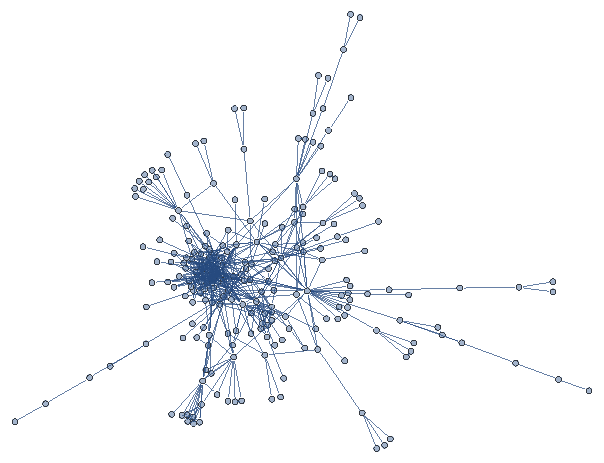
\includegraphics[width=5cm,height=4cm,angle=90]{\networksfigsdir/graph_standard.pdf}
    };
  \end{scope}
  \begin{scope}[xshift=4.5cm]
    \node [mybox] (box){
      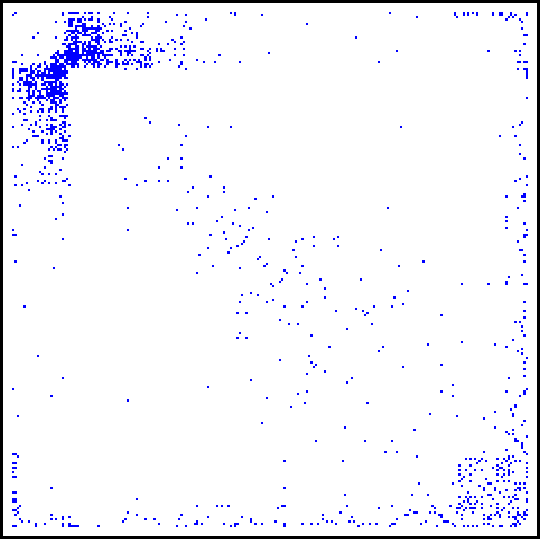
\includegraphics[width=3.5cm]{\networksfigsdir/interactome_adjacency_mathematica.pdf}

  };
  \end{scope}  
  \begin{scope}[xshift=9.2cm]
    \node [mybox] (box){
      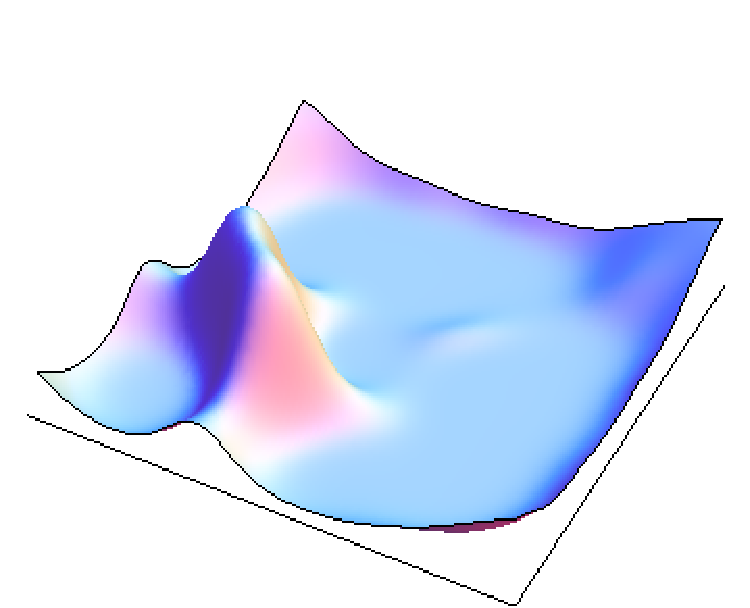
\includegraphics[width=5cm]{\networksfigsdir/graphon_listplot_bmp.pdf}
  };
  \end{scope}
\end{tikzpicture}

  \vspace{-0.5cm}
  \caption[Unsorted and sorted protein interactome and visualisation of model fit.]{Protein interactome data. 
    \emph{Left:} Interactome network. 
    \emph{Middle:} Sorted adjacency matrix. The network exhibits stochastic equivalence 
    (visible as block structure in the matrix) and homophily (concentration of points around the diagonal). 
    \emph{Right:} Maximum a posteriori estimate of the function $\AHfunction$, corresponding to the function in figure~\ref{fig:networks:graphon} (middle).
  }
  \label{fig:(R)GPLVM_Comparison}
\end{figure}

The sorted adjacency matrix and MAP estimate of $\Theta$ reveal many qualitatively different structures present in the network.
The bottom right of the adjacency matrix reveals a densely connected block of nodes; this is highlighted and visualised in figure~\ref{fig:networks:block}.
In contrast, figure~\ref{fig:networks:sparse} highlights many nodes which display patterns of transitivity although the overall connectivity is sparse.
A pair of hub nodes are also revealed as demonstrated in figure~\ref{fig:networks:hubs}.

\begin{figure}[ht]
  \centering
\begin{tikzpicture}[]
  \begin{scope}[xshift=0.0\textwidth]
    \node [mybox] (box){
      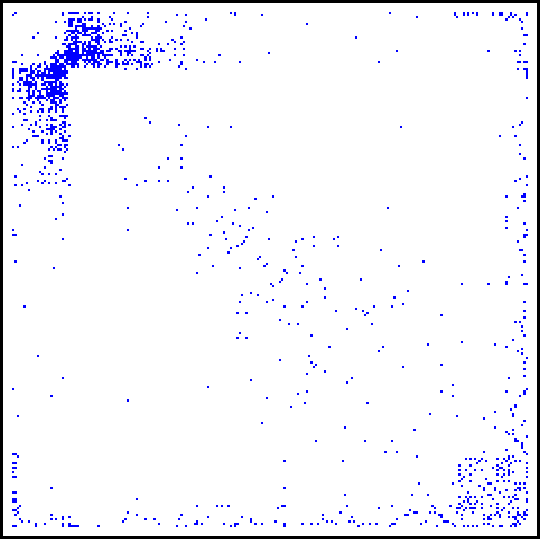
\includegraphics[width=0.45\textwidth]{\networksfigsdir/interactome_adjacency_mathematica.pdf}
    };
    \draw [dashed, ultra thick, red, opacity=0.7] (0.15\textwidth,-0.150\textwidth) -- (0.15\textwidth,-0.22\textwidth) -- (0.220\textwidth,-0.22\textwidth) -- (0.220\textwidth,-0.150\textwidth) -- (0.15\textwidth,-0.150\textwidth);
  \end{scope}  
  \begin{scope}[xshift=0.5\textwidth]
    \node [mybox] (box){
      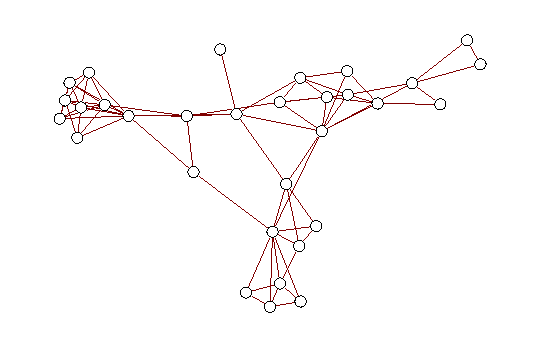
\includegraphics[width=0.45\textwidth]{\networksfigsdir/interactome_clique.pdf}
    };
  \end{scope}
\end{tikzpicture}
  \caption{A densely connected group of nodes in the protein interactome.}
  \label{fig:networks:block}
\end{figure}

\begin{figure}[ht]
  \centering
\begin{tikzpicture}[]
  \begin{scope}[xshift=0.0\textwidth]
    \node [mybox] (box){
      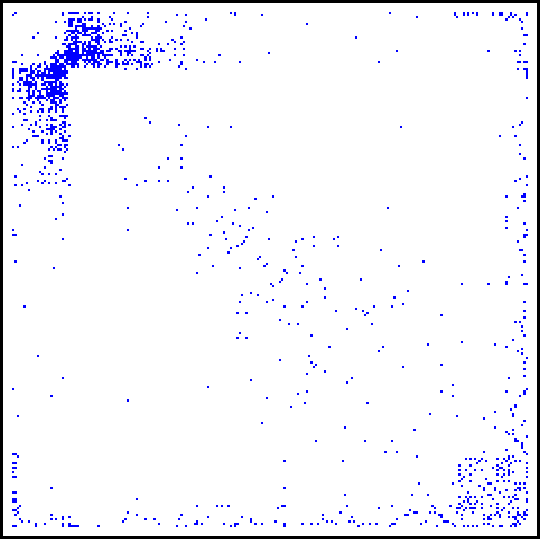
\includegraphics[width=0.45\textwidth]{\networksfigsdir/interactome_adjacency_mathematica.pdf}
    };
    \draw [dashed, ultra thick, red, opacity=0.7] (0.15\textwidth,-0.150\textwidth) -- (0.15\textwidth,+0.1\textwidth) -- (-0.1\textwidth,+0.1\textwidth) -- (-0.1\textwidth,-0.150\textwidth) -- (0.15\textwidth,-0.150\textwidth);
  \end{scope}  
  \begin{scope}[xshift=0.5\textwidth]
    \node [mybox] (box){
      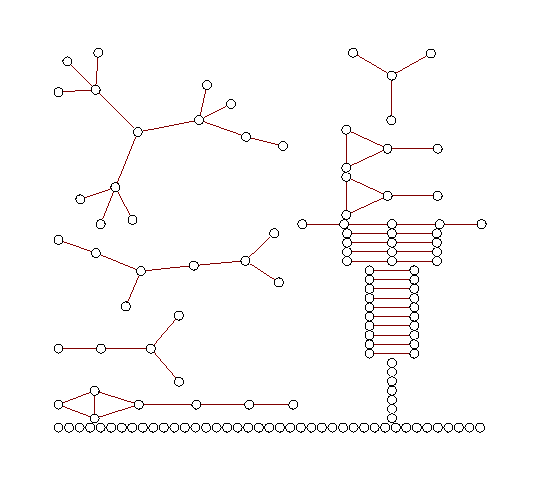
\includegraphics[width=0.45\textwidth]{\networksfigsdir/interactome_sparse.pdf}
    };
  \end{scope}
\end{tikzpicture}
  \caption[Sparsely connected nodes in the protein interactome.]{Sparsely connected nodes in the protein interactome with some transitivity (triangles).}
  \label{fig:networks:sparse}
\end{figure}

\begin{figure}[ht]
  \centering
\begin{tikzpicture}[]
  \begin{scope}[xshift=0.0\textwidth]
    \node [mybox] (box){
      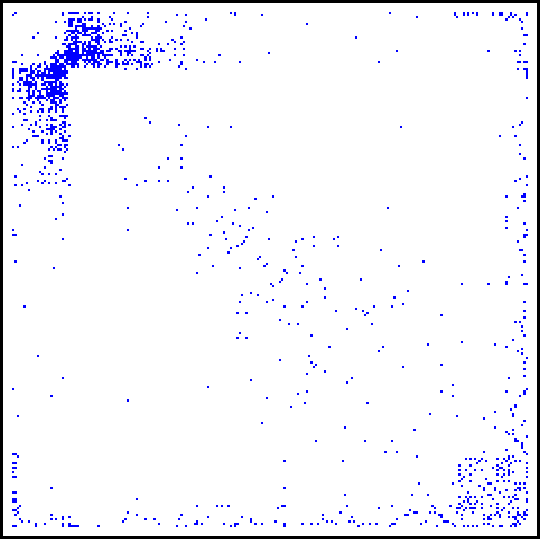
\includegraphics[width=0.45\textwidth]{\networksfigsdir/interactome_adjacency_mathematica.pdf}
    };
    \draw [dashed, ultra thick, red, opacity=0.7] (0.205\textwidth,0.22\textwidth) -- (0.205\textwidth,-0.22\textwidth) -- (0.220\textwidth,-0.22\textwidth) -- (0.220\textwidth,0.22\textwidth) -- (0.205\textwidth,0.22\textwidth);
  \end{scope}  
  \begin{scope}[xshift=0.5\textwidth]
    \node [mybox] (box){
      %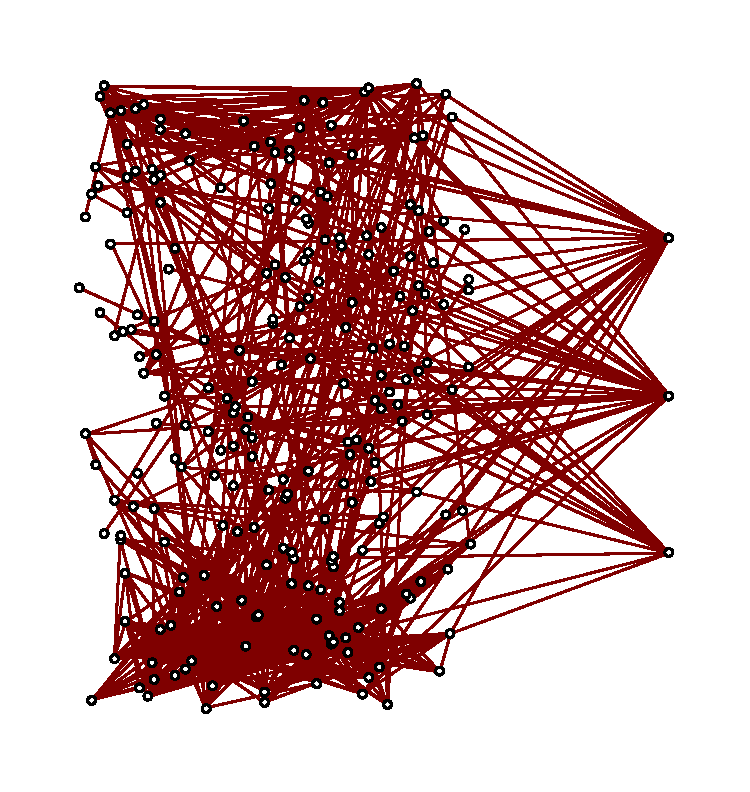
\includegraphics[width=0.45\textwidth]{\networksfigsdir/interactome_hub.pdf}
      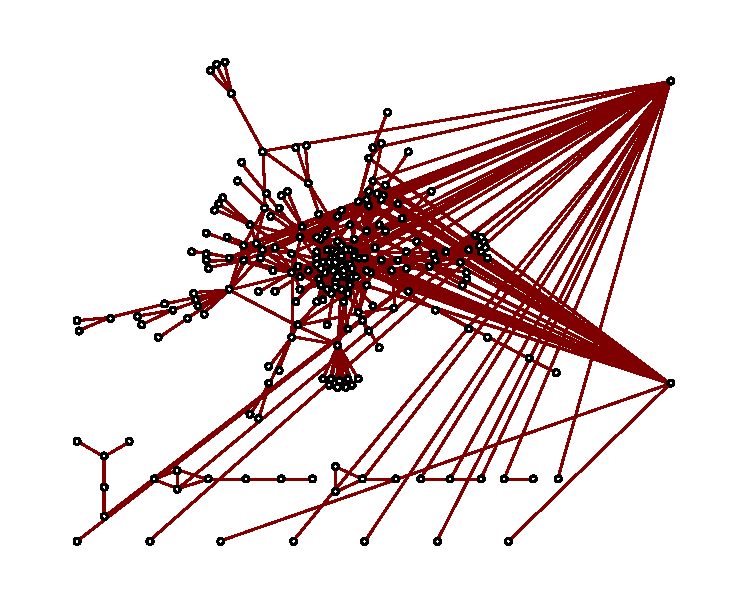
\includegraphics[width=0.45\textwidth]{\networksfigsdir/two_hub.pdf}
    };
  \end{scope}
\end{tikzpicture}
  \caption{Two hub nodes in the protein interactome.}
  \label{fig:networks:hubs}
\end{figure}

Finally, the prominent feature at the top left of the adjacency matrix is visualised in figure~\ref{fig:networks:butterfly}.
The sorted adjacency matrix has revealed three blocks of nodes which we will refer to as the left, right and top blocks according to the right hand side of figure~\ref{fig:networks:butterfly}.
Ignoring the top block, the left and right blocks are nearly bipartite.
The top block is almost a clique and is much more strongly connected to the right block than the left.
The degree distribution of the left and right blocks is also of interest; the variation is larger than expected by a block model (assuming that the probability of a link between different blocks is constant).
A more detailed analysis is currently ongoing, but the structure found by this analysis can be shown to correspond with reality; for example, the proteins on the left are almost all ribosomal subunits.\fTBD{Make sure you do this - leave many samplers going for a day each or something like that}

\begin{figure}[ht]
  \centering
\begin{tikzpicture}[]
  \begin{scope}[xshift=0.0\textwidth]
    \node [mybox] (box){
      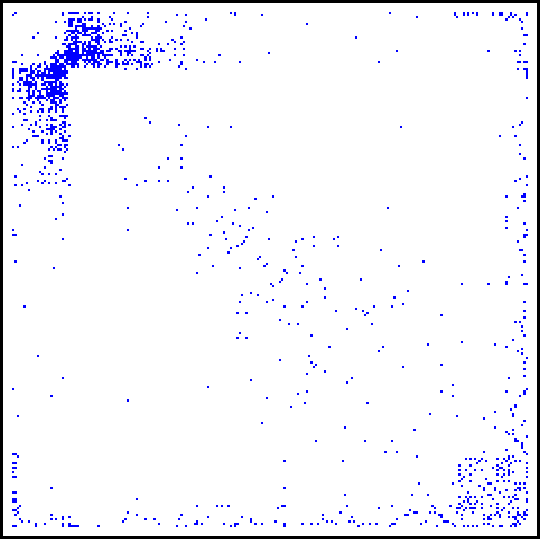
\includegraphics[width=0.45\textwidth]{\networksfigsdir/interactome_adjacency_mathematica.pdf}
    };
    \draw [dashed, ultra thick, red, opacity=0.7] (-0.22\textwidth,+0.220\textwidth) -- (-0.22\textwidth,+0.1\textwidth) -- (-0.1\textwidth,+0.1\textwidth) -- (-0.1\textwidth,+0.22\textwidth) -- (-0.22\textwidth,+0.220\textwidth);
    \draw [dotted, ultra thick, red, opacity=0.9] (-0.185\textwidth,+0.185\textwidth) -- (-0.185\textwidth,+0.16\textwidth) -- (-0.16\textwidth,+0.16\textwidth) -- (-0.16\textwidth,+0.185\textwidth) -- (-0.185\textwidth,+0.185\textwidth);
  \end{scope}  
  \begin{scope}[xshift=0.5\textwidth]
    \node [mybox] (box){
      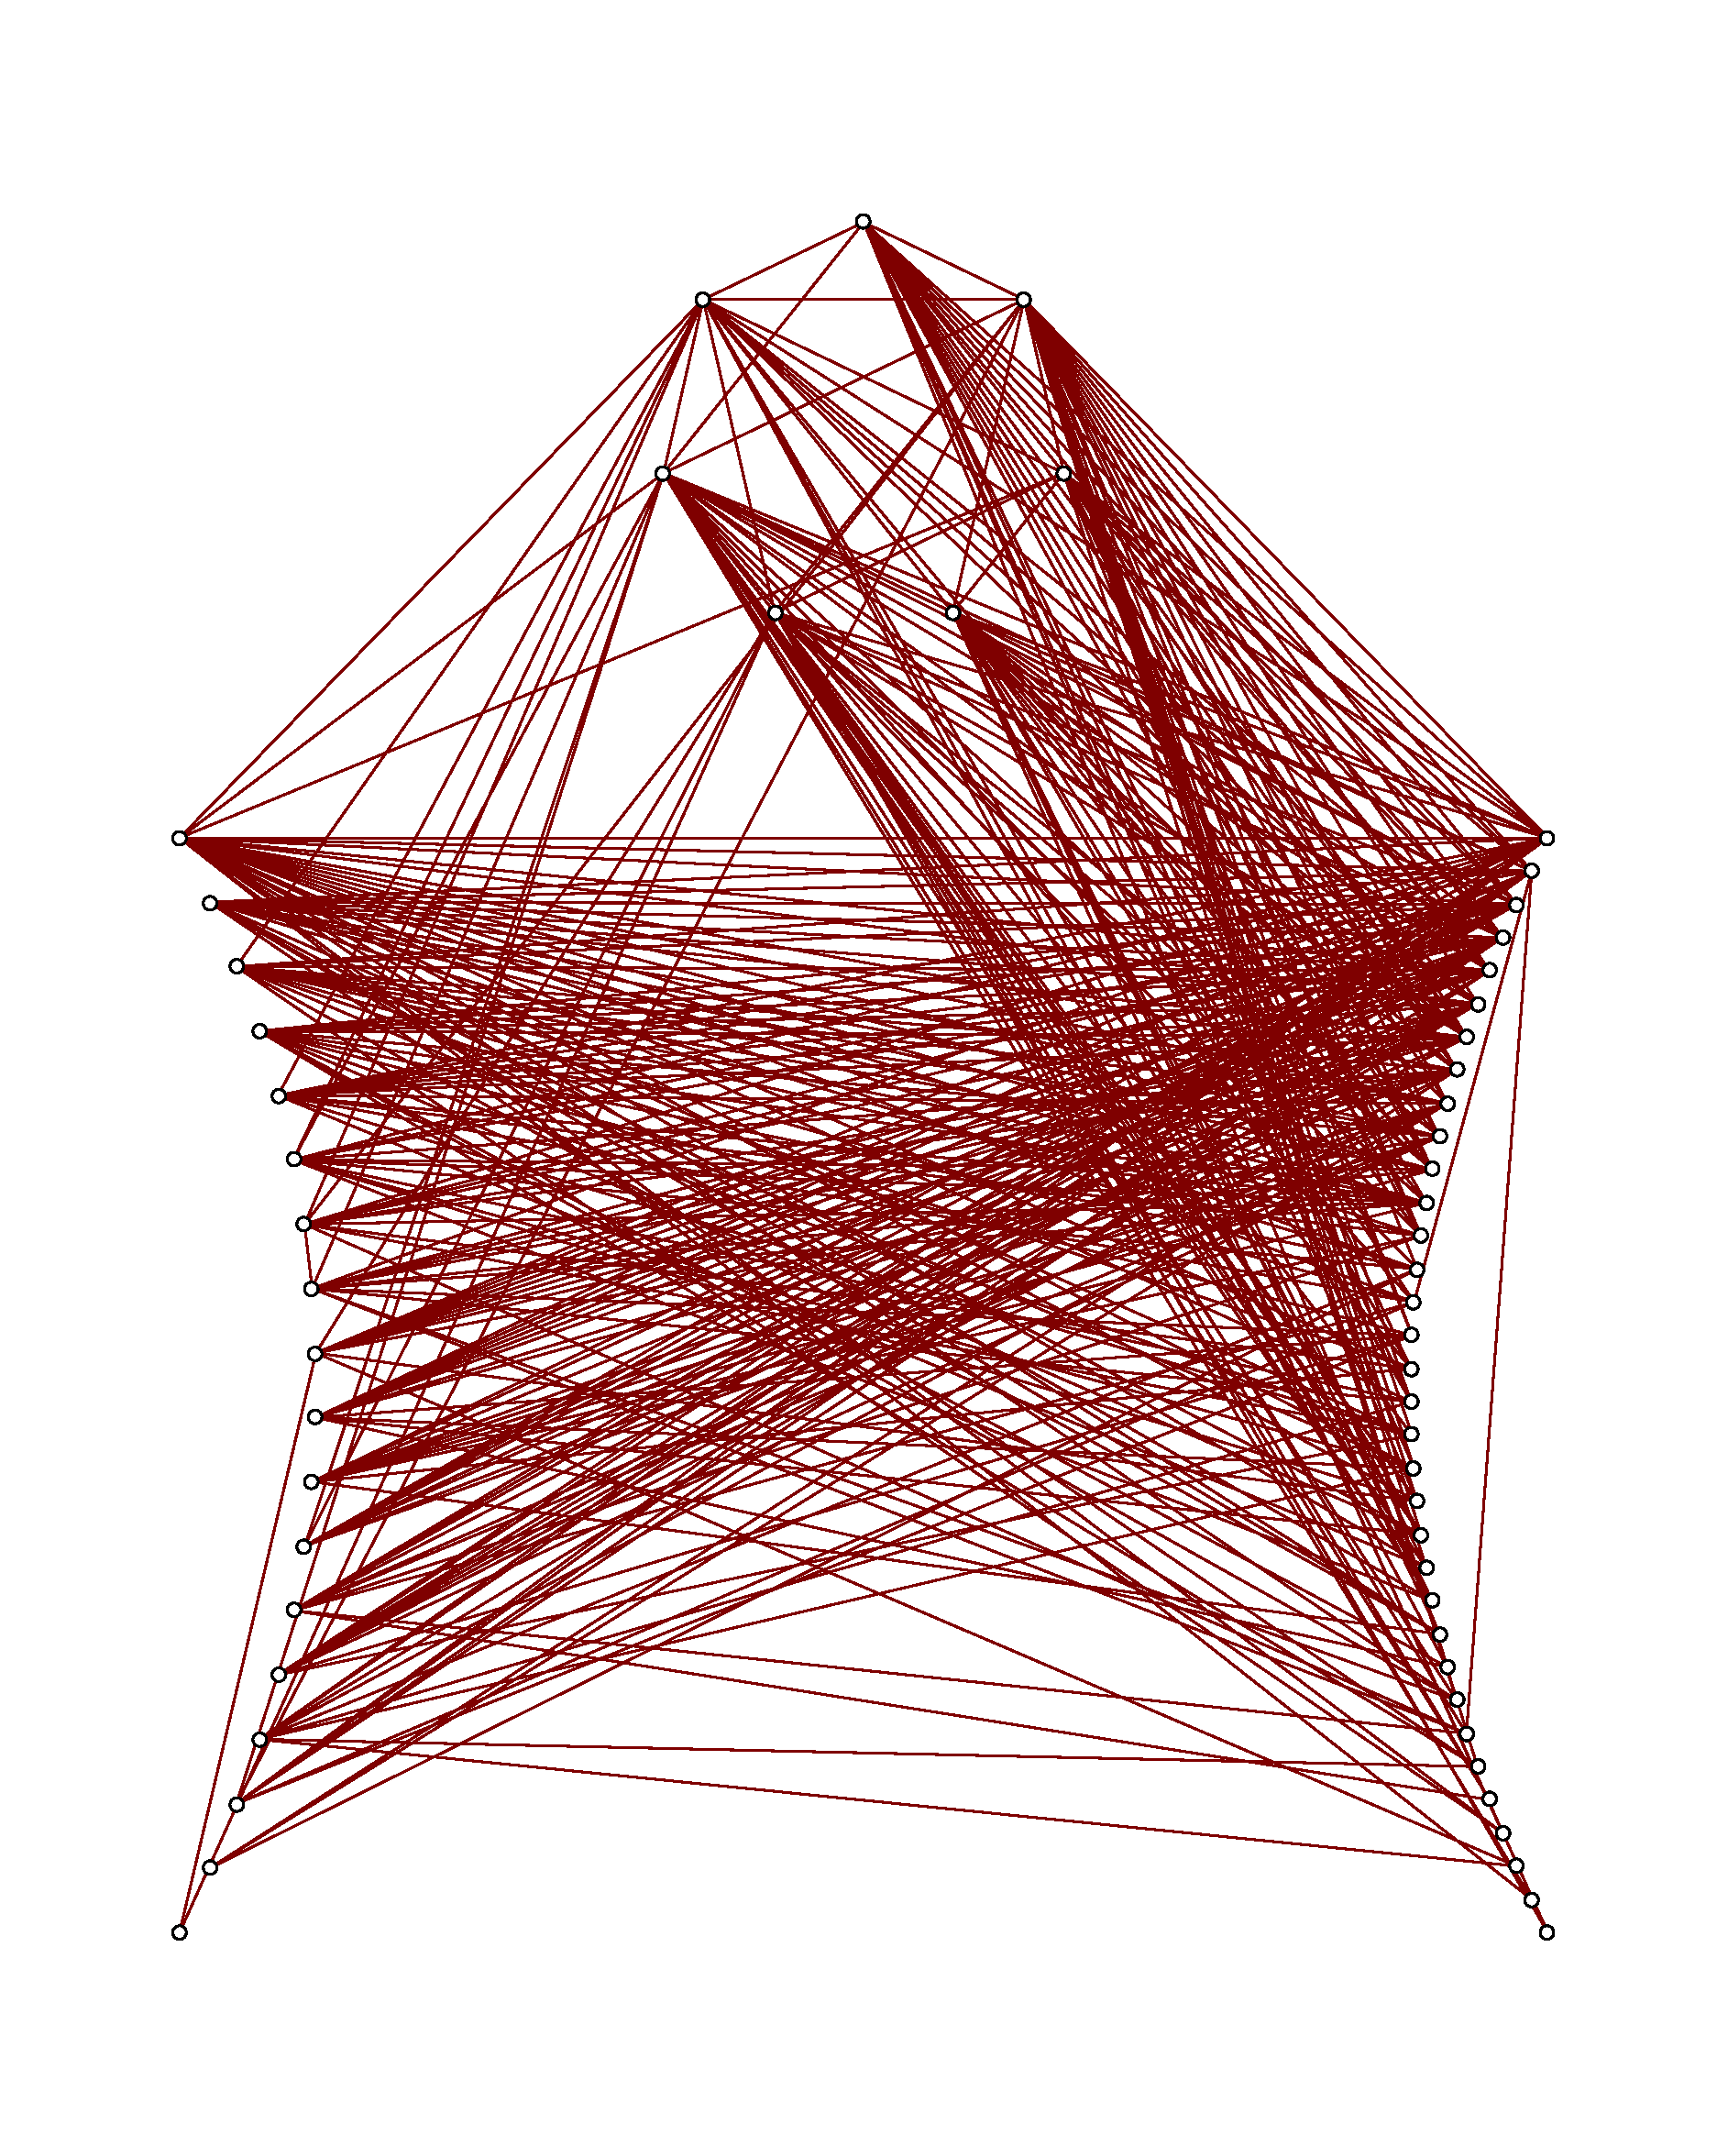
\includegraphics[width=0.45\textwidth]{\networksfigsdir/butterfly.pdf}
    };
  \end{scope}
\end{tikzpicture}
  \caption{Three groups of nodes in the protein interactome with an interesting connectivity pattern.}
  \label{fig:networks:butterfly}
\end{figure}

Similar but less complicated structures are observed in the NIPS and Highschool datasets.
Figure~\ref{fig:networks:nips} shows unsorted (left) and sorted (right) adjacency matrices for the NIPS coauthorship network.
The map embedding of the $U_i$ has identified clear block structures of densely connected groups of authors.
However, there are many authors (in the middle of the adjacency matrix) for which there is no block structure, only transitivity (coauthors of coauthors are likely to be coauthors).
Similarly, the sorted high school social network adjacency matrix in figure~\ref{fig:networks:highschool} mostly shows patterns of transitivity with most links near the diagonal.

\begin{figure}[ht]
  \centering
  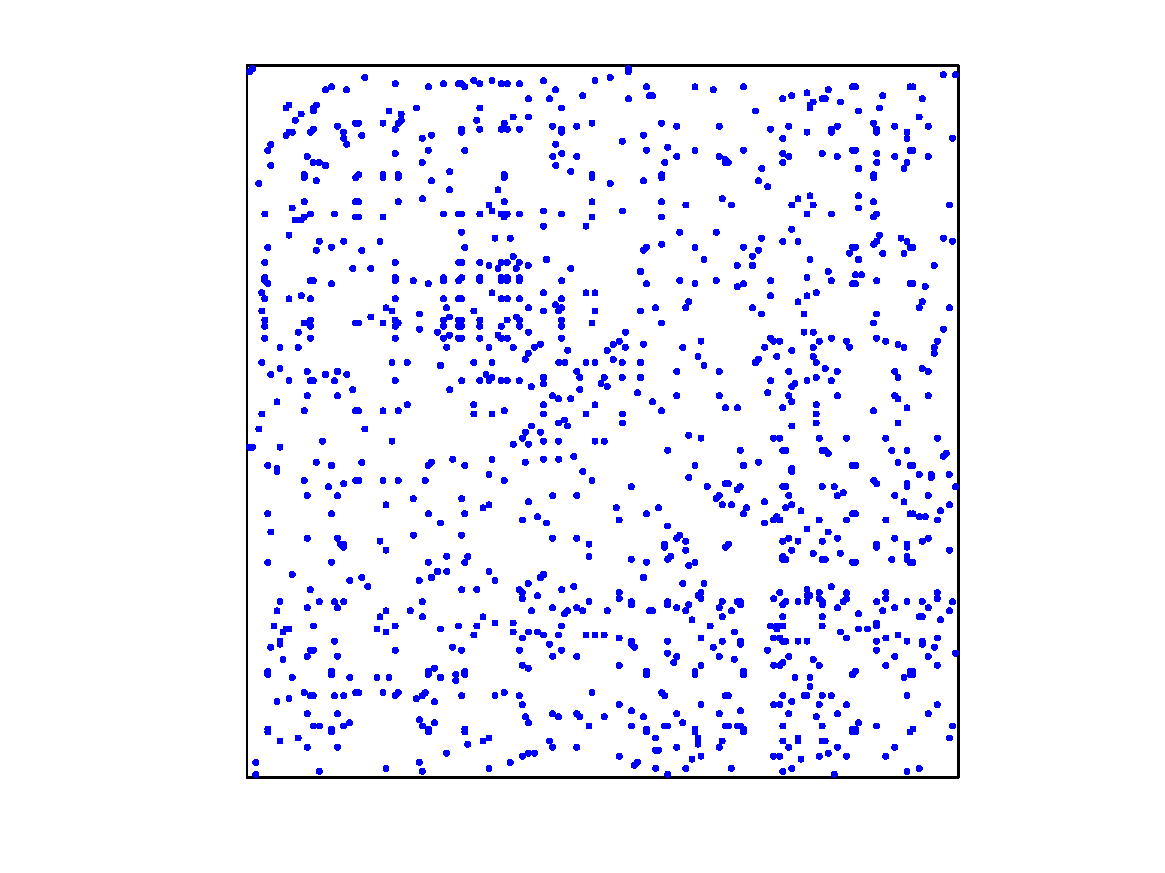
\includegraphics[width=0.45\textwidth]{\networksfigsdir/nips_unsorted}
  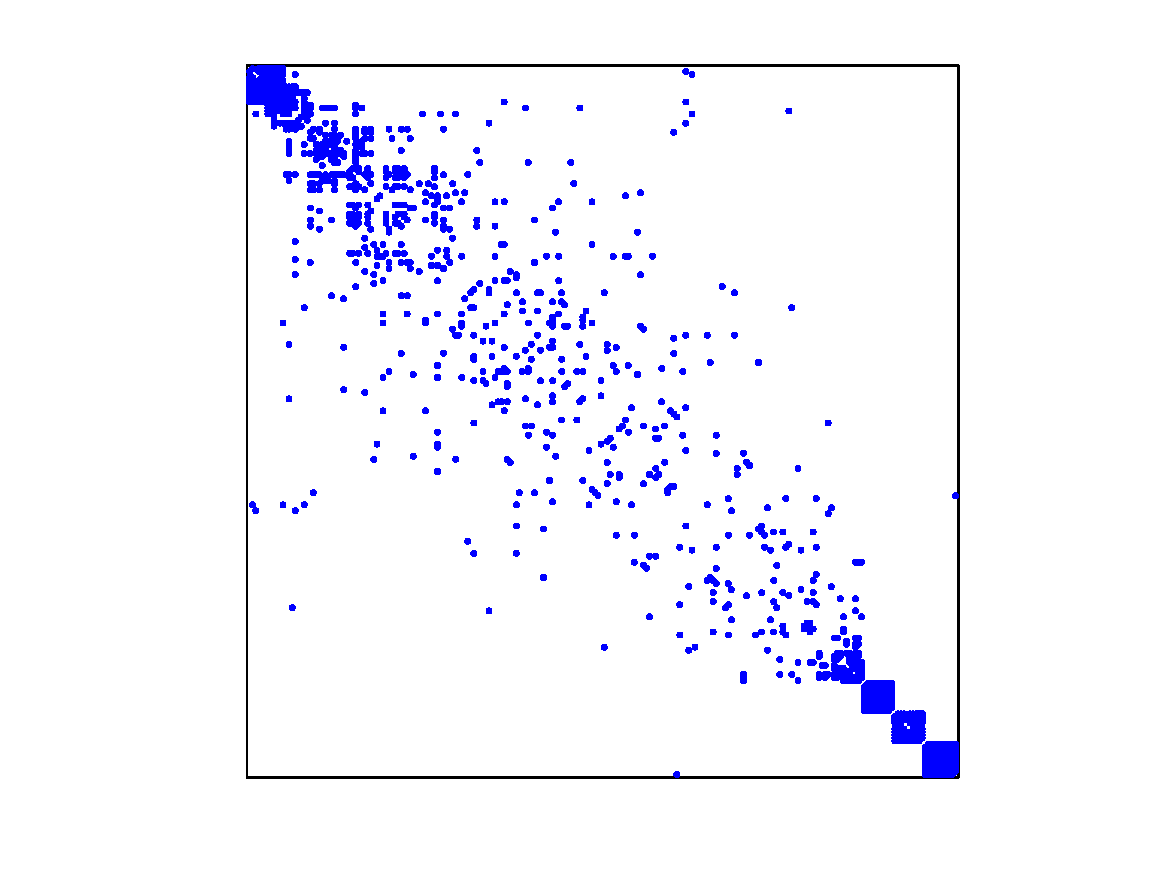
\includegraphics[width=0.45\textwidth]{\networksfigsdir/nips_sorted}
  \caption[Unsorted and sorted NIPS coauthorship adjacency matrices.]{NIPS coauthorship data. 
    \emph{Left:} Unsored adjacency matrix. 
    \emph{Middle:} Sorted adjacency matrix.
  }
  \label{fig:networks:nips}
\end{figure}

\begin{figure}[ht]
  \centering
  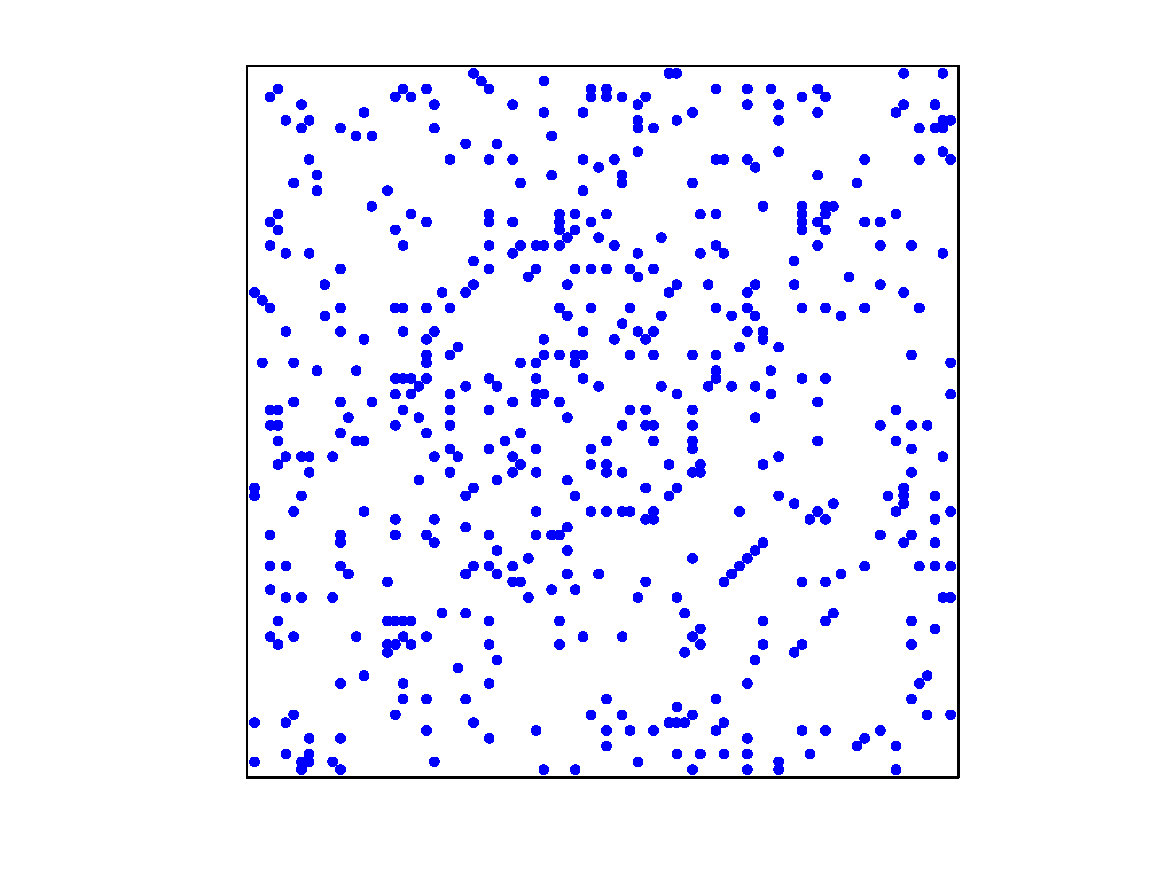
\includegraphics[width=0.45\textwidth]{\networksfigsdir/highschool_unsorted}
  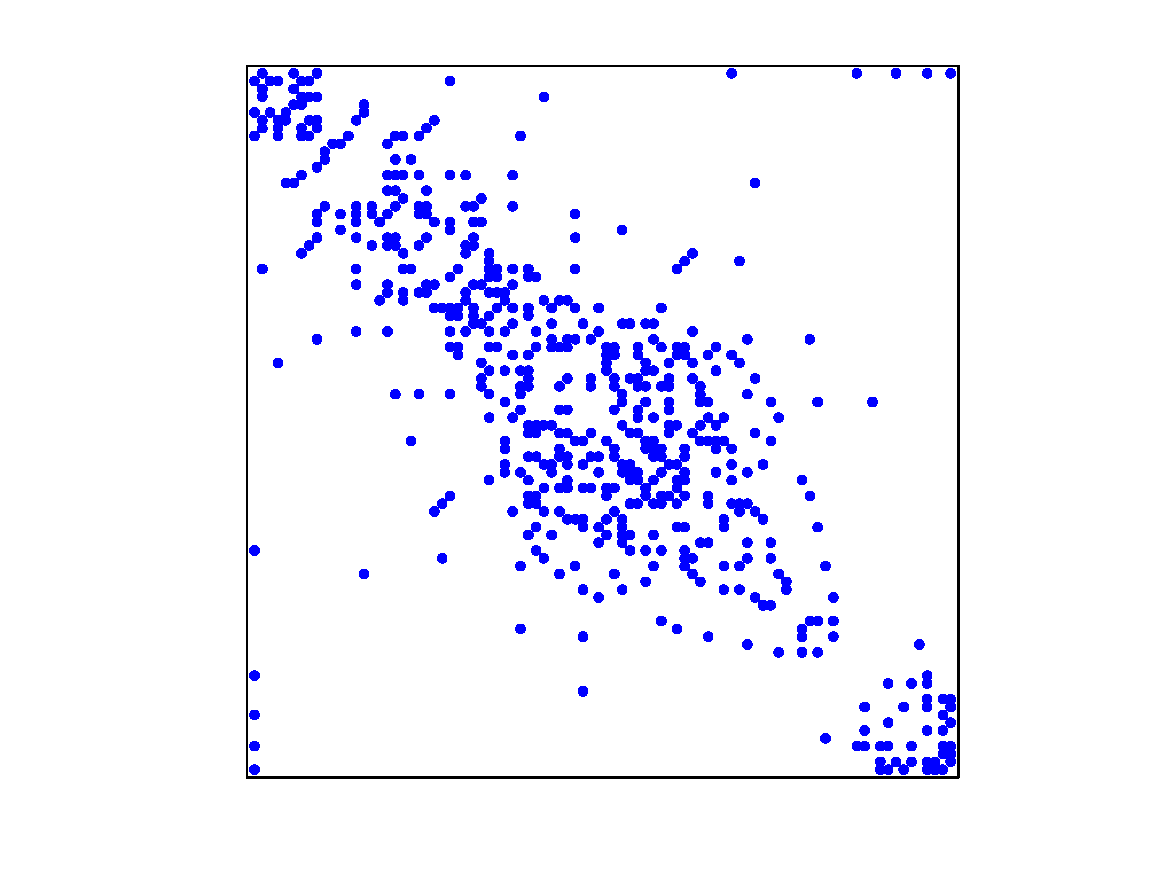
\includegraphics[width=0.45\textwidth]{\networksfigsdir/highschool_sorted}
  \caption[Unsorted and sorted highschool social network adjacency matrices.]{Highschool social network. 
    \emph{Left:} Unsored adjacency matrix. 
    \emph{Middle:} Sorted adjacency matrix.
  }
  \label{fig:networks:highschool}
\end{figure}

%\begin{rem}[Model complexity and lengthscales]
%\label{rem:lengthscale}  
%\fTBD{Needs review}
%Figure~\ref{fig:(R)GPLVM_Comparison} provides a visualisation of $\AHfunction$ when modelling the protein interactome data using 1 latent dimension.
%The most prominent feature of the plot is the smooth peak in the top left of the adjacency matrix.
%The likelihood of such a feature is sensitive to the lengthscale of the Gaussian process representation of $\AHfunction$; smaller lengthscales will encourage more complex functions and vice versa.
%It was noted in section~\ref{sec:Model} that the choice of a Gaussian process prior introduces the assumption that $\AHfunction$ is continuous.
%However, continuous functions are dense in the space of measurable functions, \ie any measurable function can be arbitrarily well approximated by a continuous one.
%The assumption of continuity is therefore not restrictive, but rather the lengthscale of the Gaussian process determines the complexity of the model a priori.
%The nonparametric prior placed on $\AHfunction$ allows the posterior to approximate any function if supported by the data, but by sampling the lengthscale we allow the model to quickly select an appropriate level of complexity.
%\end{rem}

\section{Discussion and conclusions}

There has been a tremendous amount of research into modelling matrices, arrays, graphs and relational data, but nonparametric
Bayesian modelling of such data has only recently been explored.
In most modelling circumstances, the assumption of exchangeability amongst data objects is natural and fundamental to the model.
In this case, the representation results 
\citep{Aldous1981-lg,Hoover1979-br,Kallenberg1992-gb} 
precisely map out the scope of possible probabilistic models for exchangeable arrays:
Any such model can be interpreted as a prior on random measurable functions on a suitable space.

Nonparametric Bayesian statistics provides a number of possible priors on random functions, but the Gaussian process
and its modifications are the only well-studied model for almost surely continuous functions.
For this choice of prior, our work provides a general and simple modelling approach that can be motivated directly by the
relevant representation results.
%Inference is then possible using an efficient MCMC algorithm for this model. 
The model results in both interpretable representations for networks, such as a visualisation of a protein interactome, and has 
competitive predictive performance on benchmark data.

%% There has been a tremendous amount of research into modelling matrices, arrays, graphs and relational data. 
%% In most modelling circumstances, the assumption of exchangeability amongst data objects is natural and fundamental to the model.
%% One of the contributions of this paper is to highlight fundamental results in probability theory that justify the use of latent variable models for exchangeable arrays, especially when one employs a nonparametric prior over the functions mapping from latent variables to data. We have also related our work to many other models for graphs and matrices.

%% In this paper we have used a Gaussian process prior to model random functions and have developed an efficient MCMC algorithm for this model. In doing so we have created an MCMC variant of a widely used sparse approximation for Gaussian processes.
%% Our model results in both interpretable representations for networks, such as a visualisation of a protein interactome, and has competitive predictive performance on three benchmark data sets.

\outbpdocument{
\bibliographystyle{plainnat}
\bibliography{references.bib}
}
